\documentclass[conference,a4paper]{IEEEtran}

% Vietnamese typesetting
\usepackage[T5]{fontenc}
\usepackage[utf8]{inputenc}
\usepackage{lmodern}
\usepackage{microtype}
\SetProtrusion{encoding=T5,family=lmtt}{}
\setlength{\emergencystretch}{2em}

% Mathematics
\usepackage{amsmath}
\usepackage{amssymb}

% Tables, figures, diagrams and source listings
\usepackage{graphicx}
\usepackage{pdfpages}
\graphicspath{{images/}{Title/}{figures/}}
\usepackage{booktabs}
\usepackage{longtable}
\usepackage{tabularx}
\usepackage{array}
\usepackage{multirow}
\usepackage[table]{xcolor}
\usepackage{float}
\usepackage{enumitem}
\usepackage{listings}
\usepackage{tikz}
\usetikzlibrary{arrows.meta,calc,fit,positioning,shapes.geometric}

\definecolor{HCMUSBlue}{HTML}{165A9F}
\definecolor{SoftBlue}{HTML}{EAF3FA}
\definecolor{SoftGray}{HTML}{F4F5F6}
\definecolor{CodeGreen}{HTML}{287D3C}
\definecolor{CodePurple}{HTML}{7A3E9D}
\definecolor{CodeGray}{HTML}{6A737D}
\newcolumntype{L}[1]{>{\raggedright\arraybackslash}p{#1}}
\newcolumntype{C}[1]{>{\centering\arraybackslash}p{#1}}
\newcolumntype{Y}{>{\raggedright\arraybackslash}X}
\DeclareRobustCommand{\code}[1]{\texttt{\detokenize{#1}}}
% Trình bày bảng thống nhất: tiêu đề cột hai dòng và độ lệch chuẩn cỡ nhỏ ngay sau giá trị trung bình.
\newcommand{\twoline}[2]{\begin{tabular}[b]{@{}c@{}}#1\\#2\end{tabular}}
\newcommand{\pmsd}[1]{\,{\scriptsize$\pm$#1}}

\lstdefinestyle{codeblock}{
  backgroundcolor=\color{SoftGray},
  basicstyle=\ttfamily\footnotesize,
  commentstyle=\color{CodeGreen},
  keywordstyle=\color{HCMUSBlue}\bfseries,
  stringstyle=\color{CodePurple},
  numbers=left,
  numberstyle=\tiny\color{CodeGray},
  numbersep=6pt,
  breaklines=true,
  keepspaces=true,
  showstringspaces=false,
  frame=single,
  rulecolor=\color{black!20},
  columns=fullflexible
}
\lstset{style=codeblock}

% Links, cross-references and IEEE bibliography
\usepackage[unicode,colorlinks=true,linkcolor=HCMUSBlue,citecolor=HCMUSBlue,urlcolor=HCMUSBlue]{hyperref}
\usepackage[nameinlink,noabbrev]{cleveref}
\usepackage{cite}
\crefname{section}{mục}{các mục}
\Crefname{section}{Mục}{Các mục}
\crefname{subsection}{tiểu mục}{các tiểu mục}
\Crefname{subsection}{Tiểu mục}{Các tiểu mục}
\crefname{subsubsection}{tiểu mục}{các tiểu mục}
\Crefname{subsubsection}{Tiểu mục}{Các tiểu mục}
\crefname{table}{bảng}{các bảng}
\Crefname{table}{Bảng}{Các bảng}
\crefname{figure}{hình}{các hình}
\Crefname{figure}{Hình}{Các hình}
\crefname{equation}{phương trình}{các phương trình}
\Crefname{equation}{Phương trình}{Các phương trình}
\renewcommand{\figurename}{Hình}
\renewcommand{\tablename}{Bảng}
\renewcommand{\refname}{Tài liệu tham khảo}
\renewcommand{\abstractname}{Tóm tắt}
\renewcommand{\IEEEkeywordsname}{Từ khóa}

\newcommand{\renderbibliography}{%
  \bibliographystyle{IEEEtran_nodash}% bản sao IEEEtran.bst, khoảng trang dùng gạch nối
  \bibliography{References/references}%
}

% Preserve report hierarchy in IEEE article headings:
% chapter -> section -> subsection -> subsubsection -> paragraph.
\let\IEEESection\section
\let\IEEESubsection\subsection
\let\IEEESubsubsection\subsubsection
\let\IEEEParagraph\paragraph
\makeatletter
\newcommand{\chapter}{\@ifstar{\IEEESection*}{\IEEESection}}
\renewcommand{\section}{\@ifstar{\IEEESubsection*}{\IEEESubsection}}
\renewcommand{\subsection}{\@ifstar{\IEEESubsubsection*}{\IEEESubsubsection}}
\renewcommand{\subsubsection}{\@ifstar{\IEEEParagraph*}{\IEEEParagraph}}
\makeatother

% Report metadata
\newcommand{\coursename}{Học máy với dữ liệu đồ thị}
\newcommand{\reporttitle}{Project 03: Truy vấn đa phương thức có giải thích bằng đồ thị}
\newcommand{\covertitle}{PROJECT 03: TRUY VẤN ĐA PHƯƠNG THỨC CÓ GIẢI THÍCH BẰNG ĐỒ THỊ}
\newcommand{\groupname}{Nhóm 02}
\newcommand{\studentname}{02}
\newcommand{\reportdate}{Tháng 11 năm 2026}
\newcommand{\mssv}[1]{\makebox[2.4cm][l]{#1}}
\newcommand{\studentmembers}{%
  \mssv{23120038}Lê Hoàng Mỹ Hạ \newline
  \mssv{23120106}Hàn Vũ Phương Uyên \newline
  \mssv{23120123}Trần Gia Hiển \newline
  \mssv{23120282}Chung Gia Khánh \newline
  \mssv{23127234}Nguyễn An Nghiệp%
}
\newcommand{\studentid}{\studentmembers}
\newcommand{\lecturer}{%
  TS. Lê Ngọc Thành \newline
  ThS. Huỳnh Lâm Hải Đăng%
}

\title{\reporttitle}
\IEEEspecialpapernotice{(Báo cáo đồ án môn học: \coursename{} --- Nhóm thực hiện: \groupname{})}

\author{
  \IEEEauthorblockN{Lê Hoàng Mỹ Hạ (23120038), Hàn Vũ Phương Uyên (23120106), Trần Gia Hiển (23120123)}
  \IEEEauthorblockN{Chung Gia Khánh (23120282), Nguyễn An Nghiệp (23127234)}
  \IEEEauthorblockA{Khoa Công nghệ Thông tin, Trường Đại học Khoa học Tự nhiên, ĐHQG-HCM, TP. Hồ Chí Minh, Việt Nam}
  \IEEEauthorblockA{\textit{Giảng viên hướng dẫn: TS. Lê Ngọc Thành, ThS. Huỳnh Lâm Hải Đăng}}
}

% Trang chỉ có bảng/hình toàn khổ: xếp sát từ đầu trang thay vì dàn đều theo chiều dọc.
\makeatletter
\setlength{\@dblfptop}{0pt}
\setlength{\@dblfpsep}{14pt plus 2pt}
\setlength{\@dblfpbot}{0pt plus 1fil}
\makeatother

\begin{document}

\maketitle
\begin{abstract}

Truy vấn thông tin đa phương thức giữa văn bản và hình ảnh truyền thống dựa chủ yếu trên việc so khớp vectơ đặc trưng trong không gian tiềm ẩn chung thông qua các mô hình bộ mã hóa kép như CLIP. Mặc dù đạt hiệu năng cao trong việc nắm bắt tương đồng thị giác bề mặt, cách tiếp cận thuần tương đồng vectơ này bộc lộ hai hạn chế cốt lõi: thứ nhất, mô hình hoàn toàn bỏ qua các tri thức quan hệ có cấu trúc giữa thực thể, thuộc tính và bối cảnh sự kiện; thứ hai, mô hình hoạt động như một hộp đen và không cung cấp cơ chế nội tại giải thích tại sao một kết quả cụ thể được ưu tiên xếp hạng. Đồ án này nghiên cứu và phát triển hệ thống truy vấn đa phương thức tăng cường đồ thị có khả năng giải thích dựa trên cấu trúc quan hệ, được thiết kế theo tiến trình học thuật ba cấp độ (Level 1 $\rightarrow$ Level 2 $\rightarrow$ Level 3) nhằm trả lời câu hỏi về vai trò thực chất của dữ liệu đồ thị và tính trung thực của các giải thích được sinh ra.

Ở Cấp độ 1, nghiên cứu thiết lập đường cơ sở CLIP đóng băng, xây dựng đồ thị tĩnh từ chú giải đối tượng/scene graph, áp dụng Mạng nơ-ron chú ý đồ thị GAT để tính điểm đồ thị và kết hợp rerank với điểm cosine CLIP. Kiểm chứng thực nghiệm trên tập Flickr30k Entities với 3 seed độc lập ghi nhận mô hình kết hợp CLIP + GAT đạt Mean Test MRR $\sim 0.8273$ vượt trội so với CLIP thuần ($0.7232$). Tuy nhiên, phân tích triệt tiêu ablation study cho thấy cấu hình không cạnh (adapter với self-loops) cũng đóng góp đáng kể, chứng minh không thể quy toàn bộ phần cải thiện cho cấu trúc quan hệ nếu thiếu kiểm soát thực nghiệm chặt chẽ.

Ở Cấp độ 2, nghiên cứu mở rộng sang đồ thị tri thức đa phương thức MMKG phức tạp trên DB15K và FB15k-237, triển khai cơ chế dung hợp đặc trưng AdaMF-based và phân tích chuyên sâu hiệu năng trên 20 truy vấn đánh giá phân tách rõ nhánh trực tiếp và gián tiếp. Bằng chứng audit độc lập trên DB15K (seed 2027) xác nhận mô hình Full Graph đạt Test MRR $0.4145$ (Recall@10 đạt $0.5556$, indirect MRR đạt $0.3164$), cải thiện vượt bậc so với baseline CLIP thuần ($0.2577$) và vượt cấu hình Shuffled Edges v2 ($0.3156$). Báo cáo ghi nhận minh bạch đặc điểm kỹ thuật của giao thức tạo đồ thị hoán đổi cạnh bảo toàn bậc và kiểm soát rò rỉ tập kiểm thử.

Ở Cấp độ 3, nghiên cứu xây dựng cơ chế trích xuất đường đi và đồ thị con giải thích bắt nguồn trực tiếp từ cơ chế tính điểm xếp hạng, thiết lập quy trình đo lường định lượng fidelity, validity và sparsity trên các trường hợp truy vấn thành công và thất bại điển hình, đồng thời đánh giá khả năng chuyển giao trên tập dữ liệu MMKG tự xây. Báo cáo giữ nguyên tính trung thực học thuật bằng việc phân định ranh giới rõ ràng giữa các kết quả đã được xác minh bằng artifact thực tế và các hạng mục đang trong quá trình hoàn thiện thực nghiệm.

\end{abstract}

\begin{IEEEkeywords}
Truy vấn đa phương thức; MMKG; CLIP; GAT; Dung hợp AdaMF; Graph Explainability; Fidelity.
\end{IEEEkeywords}


\chapter{Giới thiệu}
\label{chap:introduction}

\section{Bối cảnh nghiên cứu}
\label{sec:research-background}

Trong kỷ nguyên bùng nổ dữ liệu số, nhu cầu tìm kiếm và truy hồi thông tin tương tác giữa nhiều phương thức biểu diễn -- đặc biệt là giữa văn bản và hình ảnh -- đã trở thành một trong những bài toán trọng tâm của trí tuệ nhân tạo. Sự xuất hiện của các mô hình ngôn ngữ--thị giác tiền huấn luyện trên quy mô lớn như CLIP \cite{radford2021clip} đã mở ra bước đột phá vượt bậc. Bằng cách chiếu các đặc trưng biểu diễn của văn bản và hình ảnh vào cùng một shared latent space, các hệ thống truy vấn có thể xác định mức độ phù hợp thông qua độ đo cosine similarity giữa hai vectơ biểu diễn một cách hiệu quả và có khả năng khái quát hóa dạng zero-shot ấn tượng.

Tuy nhiên, trong các tình huống thực tế, thế giới quan không chỉ đơn thuần là các mảng điểm ảnh hay các từ ngữ xuất hiện độc lập, mà luôn mang cấu trúc quan hệ ngữ nghĩa chặt chẽ. Một bức ảnh luôn chứa đựng nhiều thực thể với các mối liên kết không gian, chức năng hoặc hành động tương hỗ (ví dụ: một đứa trẻ đang đá bóng trên sân cỏ). Biểu diễn vectơ dày đặc của CLIP tuy nắm bắt xuất sắc diện mạo tổng thể nhưng thường gặp khó khăn trong việc hiểu rõ cấu trúc cú pháp quan hệ phức tạp và các tri thức suy luận ngầm định không xuất hiện trực tiếp dưới dạng đặc trưng thị giác bề mặt.


\section{Phát biểu bài toán}
\label{sec:problem-statement}

Mặc dù mô hình truy hồi dựa trên tương đồng không gian tiềm ẩn đạt tốc độ tính toán nhanh nhờ các thư viện chỉ mục vectơ như FAISS \cite{johnson2019faiss}, mô hình này tồn tại hai hạn chế mang tính cố hữu:
\begin{enumerate}[label=(\arabic*)]
  \item \textbf{Thiếu hụt khả năng mô hình hóa tri thức quan hệ:} Trong các truy vấn gián tiếp đòi hỏi suy luận logic hoặc liên kết đa chặng (ví dụ: truy vấn \textit{"a child playing football"} khi ảnh chỉ nhận diện được hai nhãn đối tượng là \textit{"ball"} và \textit{"field"}), mô hình dựa trên tương đồng vectơ thuần túy thường bỏ sót kết quả đúng do thiếu vắng đường đi kết nối tri thức \textit{child -- plays -- football}.
  \item \textbf{Thiếu vắng tính Explainability:} Mô hình hộp đen chỉ trả về một giá trị tương đồng vô hướng, hoàn toàn không cho người dùng biết vì sao một hình ảnh lại được xếp hạng cao hơn hình ảnh khác, hoặc thành phần tri thức cụ thể nào trong ảnh đã đóng góp vào quyết định xếp hạng.
\end{enumerate}
Do đó, bài toán đặt ra cho đề tài là: \textit{Xây dựng hệ thống truy hồi đa phương thức kết hợp thông tin quan hệ từ đồ thị (Scene Graph và MMKG) nhằm cải thiện chất lượng xếp hạng kết quả, đồng thời sinh ra các giải thích trực quan dưới dạng quan hệ, đường đi hoặc đồ thị con có tính trung thực cao bắt nguồn từ chính cơ chế tính điểm của mô hình.}


\section{Mục tiêu và câu hỏi nghiên cứu}
\label{sec:research-objectives}

Đồ án được thiết kế theo một cấu trúc học thuật chặt chẽ, tiến triển qua ba giai đoạn kế thừa lẫn nhau tương ứng với ba cấp độ nghiên cứu. Mỗi cấp độ tập trung giải quyết một câu hỏi khoa học xác định:

\begin{itemize}
  \item \textbf{Cấp độ 1:} Tập trung vào câu hỏi nghiên cứu \textbf{RQ1}: \textit{"Việc tích hợp cấu trúc đồ thị tĩnh thông qua mạng nơ-ron đồ thị GAT có thực sự cải thiện độ chính xác truy hồi so với baseline CLIP thuần túy hay không, và phần cải thiện này đến từ cấu trúc đồ thị hay từ việc gia tăng tham số của projection adapter?"}
  \item \textbf{Cấp độ 2:} Tập trung vào câu hỏi nghiên cứu \textbf{RQ2}: \textit{"Khi mở rộng sang MMKG đa quan hệ và áp dụng cơ chế AdaMF-based feature fusion, tri thức quan hệ đóng góp như thế nào vào việc nâng cao chất lượng truy vấn, đặc biệt là đối với các truy vấn gián tiếp đòi hỏi suy luận liên kết?"}
  \item \textbf{Cấp độ 3:} Tập trung vào câu hỏi nghiên cứu \textbf{RQ3}: \textit{"Các đường đi và đồ thị con giải thích được trích xuất từ cơ chế tính điểm đồ thị có đạt fidelity với hành vi xếp hạng của mô hình hay không, và giải pháp đề xuất có khả năng chuyển giao sang tập đồ thị đa phương thức tự xây cho miền đặc thù hay không?"}
\end{itemize}

Mối quan hệ phụ thuộc logic giữa ba câu hỏi nghiên cứu được thể hiện rõ: RQ1 thiết lập nền tảng đo lường hiệu quả của đồ thị và kiểm soát kiểm thử triệt tiêu; RQ2 nâng cấp biểu diễn đồ thị sang không gian đa quan hệ MMKG và giải quyết bài toán truy vấn gián tiếp; RQ3 đi sâu vào bản chất minh bạch của quá trình ra quyết định ở hai cấp độ trước và kiểm tra tính tổng quát hóa trong môi trường dữ liệu mới.


\section{Phạm vi nghiên cứu và đóng góp}
\label{sec:research-scope}

\subsection{Phạm vi nghiên cứu}
Nghiên cứu tập trung vào bài toán truy hồi Text-to-Image làm nhánh thực nghiệm chính theo đúng đặc tả chuẩn của đề bài. Nhánh mở rộng Image-to-Text và Text-to-Video được định vị ở mức khảo sát mở rộng. Các bộ dữ liệu chính được sử dụng gồm Visual Genome, DB15K và FB15k-237, kết hợp với tập dữ liệu khảo sát MMKG tự xây miền hẹp.

\subsection{Tóm tắt đóng góp chính}
Các đóng góp chính của đồ án bao gồm:
\begin{enumerate}
  \item Xây dựng pipeline truy hồi đa phương thức chuẩn hóa tích hợp CLIP và đồ thị, bảo đảm giao thức chia tập dữ liệu nghiêm ngặt chống data leakage và kiểm soát seed ngẫu nhiên.
  \item Triển khai và đánh giá thực nghiệm mô hình Graph Attention Network (GAT) trên Visual Genome, thực hiện ablation study kiểm chứng vai trò của cấu trúc cạnh bằng các đối chứng không cạnh và cạnh ngẫu nhiên.
  \item Hiện thực hóa mô hình dung hợp đa phương thức dựa trên AdaMF trên hai tập chuẩn MMKG (DB15K và FB15k-237), phân tích chuyên sâu sự khác biệt hiệu năng giữa 20 truy vấn trực tiếp và gián tiếp.
  \item Thiết kế giao thức đánh giá giải thích định lượng thông qua ba chỉ số: Fidelity, Validity và Sparsity, kèm theo phân tích định tính trên các trường hợp thành công và thất bại.
  \item Khảo sát khả năng chuyển giao trên tập dữ liệu MMKG tự xây (tiếng Việt miền hẹp) và ghi nhận minh bạch các giới hạn thực nghiệm.
\end{enumerate}

\chapter{Cơ sở lý thuyết và công trình liên quan}
\label{chap:related-work}

\section{Truy vấn thông tin đa phương thức}
\label{sec:multimodal-retrieval}

CLIP~\cite{radford2021clip} mã hóa câu truy vấn $q$ và ảnh $v_i$ vào cùng không gian vectơ. Với hai embedding đã chuẩn hóa L2 là $e_q$ và $e_{v_i}$, độ tương đồng giữa truy vấn và ảnh được tính như sau:
\begin{equation}
  S_{\text{CLIP}}(q,v_i)=\cos(e_q,e_{v_i})=e_q^\top e_{v_i}.
  \label{eq:clip-similarity}
\end{equation}
Các chỉ số MRR và Recall@$K$ được trình bày ở Mục~\ref{sec:metrics}.

\section{Học biểu diễn đồ thị}
\label{sec:graph-representation-learning}

Đồ thị cảnh của Visual Genome~\cite{krishna2017visualgenome} biểu diễn đối tượng bằng đỉnh và quan hệ giữa các đối tượng bằng cạnh. Các mô hình GCN, GraphSAGE và GAT đều tổng hợp thông tin từ láng giềng~\cite{kipf2017gcn,hamilton2017graphsage,velickovic2018gat}. Ở cấp độ 1, nhóm dùng GAT để học trọng số khi tổng hợp đặc trưng của các đỉnh.

\section{Cải thiện truy vấn bằng đồ thị}
\label{sec:graph-enhanced-retrieval}

CLIP lấy các ảnh ứng viên có điểm tương đồng cao. Mô hình đồ thị bổ sung điểm về mức phù hợp của ảnh với quan hệ trong truy vấn. điểm tương đồng CLIP và điểm đồ thị được chuẩn hóa z-score theo từng truy vấn trước khi kết hợp với trọng số $\alpha_{\mathrm{CLIP}}$ chọn trên tập validation. Chi tiết triển khai ở hai cấp độ được trình bày tại Mục~\ref{sec:level1-methodology} và Mục~\ref{sec:level2-methodology}.

\section{Đồ thị tri thức đa phương thức và công trình liên quan}
\label{sec:advanced-mmkg-methods}

Đồ thị tri thức đa phương thức gắn ảnh và văn bản với các thực thể trong bộ ba $(h,r,t)$~\cite{liu2019mmkg}. Với truy vấn gián tiếp, hệ thống sử dụng quan hệ $r$ và một thực thể đã biết, sau đó thay vị trí còn thiếu trong $(h,r,?)$ hoặc $(?,r,t)$ bằng thực thể tương ứng với từng ảnh ứng viên để đánh giá mức độ phù hợp.

AdaMF học trọng số để kết hợp đặc trưng cấu trúc, ảnh và văn bản của mỗi thực thể~\cite{adamfmat2024}. RotatE~\cite{sun2019rotate} chấm bộ ba dựa trên khoảng cách giữa đầu sau phép quay theo quan hệ và đuôi. NativE khai thác trọng số theo quan hệ để xử lý sự không cân bằng giữa các phương thức~\cite{native2024sigir}.

Ở cấp độ 2, nhóm sử dụng AdaMF để kết hợp đặc trưng từ nhiều nguồn và bộ chấm điểm RotatE để đánh giá mức độ phù hợp của các bộ ba trong đồ thị tri thức. Thành phần huấn luyện đối kháng MAT không được sử dụng trong cấu hình này (hệ số bằng 0). DB15K dùng SigmoidLoss trên bộ ba dương và âm. FB15K-237-IMG dùng cross-entropy để xếp ảnh đúng lên trên các ảnh âm của cùng truy vấn.

\section{Truy vấn đồ thị có khả năng giải thích}
\label{sec:explainable-retrieval}

GNNExplainer và SubgraphX tìm đồ thị con để giải thích dự đoán của GNN~\cite{ying2019gnnexplainer,yuan2021subgraphx}. Với mô hình nhúng đồ thị tri thức, Kelpie đánh giá ảnh hưởng của bộ ba bằng cách học lại embedding sau can thiệp~\cite{rossi2022kelpie}.

Nhóm đánh giá mức độ ảnh hưởng của các quan hệ được dùng để giải thích bằng cách lần lượt loại bỏ, chỉ giữ lại hoặc làm nhiễu chúng trong đồ thị, sau đó tính lại điểm của ảnh được xếp hạng cao nhất~\cite{amara2022graphframex}. $\mathrm{Fid}^{+}$ đo mức giảm tương đối của xác suất xếp hạng khi bỏ bằng chứng, còn $\mathrm{Fid}^{-}$ đo mức giảm khi chỉ giữ bằng chứng. Sparsity đo tỷ lệ phần tử ứng viên bị lược bỏ. PN và PS lần lượt đo tỷ lệ ảnh mất hạng nhất khi bỏ bằng chứng và giữ hạng nhất khi chỉ giữ bằng chứng.

\chapter{Phương pháp đề xuất và triển khai}
\label{chap:methodology}

\section{Sơ đồ nghiên cứu tổng quát}
\label{sec:overall-framework}

Quy trình nghiên cứu tổng quát của đồ án được xây dựng dưới dạng một kiến trúc đa tầng tích hợp, kết nối xuyên suốt ba cấp độ thực hiện từ bài toán cơ sở đến giải pháp nâng cao và giải thích quyết định. Hệ thống nhận đầu vào là câu truy vấn văn bản $q$ và một không gian tìm kiếm hình ảnh quy mô lớn. 

Khung làm việc bao gồm ba khối chức năng dùng chung và ba nhánh thuật toán tương ứng:
\begin{enumerate}
  \item \textbf{Khối trích xuất đặc trưng cơ sở:} Sử dụng mô hình CLIP (frozen ViT-B/32) để mã hóa toàn bộ cơ sở dữ liệu ảnh và sinh biểu diễn vectơ cho câu truy vấn đầu vào.
  \item \textbf{Khối lọc ứng viên sơ bộ:} Tận dụng tìm kiếm cosine similarity nhanh nhằm thu hẹp không gian tìm kiếm xuống tập top-$k$ candidates tiềm năng nhất.
  \item \textbf{Khối chấm điểm và xếp hạng lại:} Áp dụng GAT trên đồ thị tĩnh (Level 1) hoặc mô hình dung hợp thích nghi AdaMF trên MMKG (Level 2).
  \item \textbf{Khối giải thích và kiểm chứng độ tin cậy:} Phân rã đường đi và trọng số chú ý để trích xuất đồ thị con chứng minh, sau đó tiến hành kiểm tra fidelity bằng phương pháp can thiệp làm nhiễu đồ thị.
\end{enumerate}


\section{Cấp độ 1: Mô hình cơ sở và truy vấn tăng cường đồ thị}
\label{sec:level1-methodology}

\subsection{Mô hình cơ sở CLIP (Baseline)}

Trên tập dữ liệu Visual Genome, nhóm sử dụng mô hình CLIP ViT-B/32
với trọng số tiền huấn luyện từ OpenAI làm mô hình cơ sở (baseline)
để đánh giá hiệu quả truy vấn khi chưa sử dụng thông tin đồ thị.

Với mỗi câu truy vấn văn bản $q$, CLIP sử dụng bộ mã hóa văn bản
để tạo vectơ đặc trưng tương ứng. Tương tự, mỗi ảnh $v_i$ trong
tập dữ liệu được biểu diễn bằng một vectơ đặc trưng thông qua bộ
mã hóa hình ảnh. Hai vectơ này nằm trong cùng một không gian biểu
diễn, cho phép tính mức độ tương đồng giữa câu truy vấn và hình
ảnh bằng cosine similarity theo công thức~\eqref{eq:clip-similarity}.
Các ảnh sau đó được sắp xếp theo điểm tương đồng giảm dần,
trong đó ảnh có điểm cao hơn được xem là phù hợp hơn với truy vấn.

Trong quá trình thực nghiệm, toàn bộ tham số của CLIP được giữ
cố định, không thực hiện huấn luyện bổ sung (fine-tuning).
Kết quả truy vấn từ mô hình này được sử dụng làm cơ sở so sánh
với phương pháp kết hợp thông tin đồ thị ở các bước tiếp theo.


\subsection{Xây dựng đồ thị tĩnh}
\label{sec:static-graph}

Trên tập dữ liệu Visual Genome, nhóm xây dựng đồ thị từ các
scene graph có sẵn. Mỗi ảnh được biểu diễn bằng một đồ thị
riêng biệt $G_i=(V_i,E_i)$, trong đó $V_i$ là tập đỉnh và
$E_i$ là tập cạnh. Các đồ thị được xây dựng độc lập, không
có cạnh kết nối giữa các ảnh khác nhau.

\textbf{Biểu diễn các đỉnh.}
Mỗi đồ thị gồm một đỉnh đại diện cho toàn bộ ảnh và các đỉnh
đại diện cho những thực thể xuất hiện trong ảnh. Đỉnh ảnh
được khởi tạo bằng vectơ đặc trưng 512 chiều trích xuất từ
ảnh gốc. Đối với mỗi đỉnh thực thể, nhóm sử dụng tên thực
thể đã chuẩn hóa để tạo vectơ đặc trưng văn bản 512 chiều.
Tất cả các đặc trưng đều được trích xuất bằng CLIP
\texttt{ViT-B-32}, với trọng số tiền huấn luyện
\texttt{openai}, và được giữ cố định trong quá trình
huấn luyện GAT.

\textbf{Xây dựng các cạnh.}
Các cạnh trong đồ thị được chia thành hai nhóm. Nhóm thứ
nhất kết nối đỉnh ảnh với các đỉnh thực thể thông qua
quan hệ \texttt{contains}, thể hiện rằng thực thể đó
xuất hiện trong ảnh:

\[
v_{\mathrm{image}}
\xrightarrow{\mathrm{contains}}
v_{\mathrm{entity}}.
\]

Nhóm thứ hai biểu diễn quan hệ giữa các thực thể, được
lấy trực tiếp từ scene graph của Visual Genome. Chẳng
hạn, quan hệ \texttt{wearing} mô tả một thực thể đang
mặc một vật, trong khi \texttt{holding} thể hiện hành
động cầm hoặc giữ một vật. Các quan hệ khác bao gồm
\texttt{on}, \texttt{has}, \texttt{in}, v.v.

Các quan hệ trong scene graph ban đầu đều có hướng.
Chẳng hạn, quan hệ \texttt{holding} nối từ thực thể
\texttt{man} đến \texttt{ball}, thể hiện một người
đang cầm quả bóng. Nếu chỉ giữ cạnh này, thông tin
chỉ được truyền từ \texttt{man} sang \texttt{ball}
theo hướng của cạnh. Vì vậy, nhóm bổ sung một cạnh
ngược từ \texttt{ball} về \texttt{man}, giúp GAT
tổng hợp thông tin từ cả hai phía của quan hệ.

Mỗi cạnh được biểu diễn bằng vectơ đặc trưng 512
chiều của tên quan hệ, trích xuất bằng bộ mã hóa
văn bản CLIP. Ngoài ra, biến nhị phân
\texttt{edge\_is\_reverse} được sử dụng để phân biệt
cạnh gốc và cạnh được bổ sung. Danh sách các loại
quan hệ được xác định từ tập huấn luyện; những quan
hệ chưa từng xuất hiện trong tập này được gán nhãn
\texttt{UNK\_REL}.

\textbf{Xử lý self-loop.}
GAT được cấu hình \texttt{add\_self\_loops=False},
nghĩa là mô hình không tự động bổ sung self-loop.
Các self-loop ngữ nghĩa có sẵn trong dữ liệu
Visual Genome vẫn được giữ lại.

\textbf{Ví dụ minh họa.}
Đối với ảnh có mã định danh \texttt{61512} trong
Visual Genome, đồ thị gồm một đỉnh ảnh, 18 đỉnh
thực thể và 27 cạnh gốc. Trong đó, 18 cạnh
\texttt{contains} kết nối đỉnh ảnh với các thực thể,
còn những cạnh khác mô tả quan hệ giữa các thực thể,
chẳng hạn như:

\[
\begin{aligned}
\mathrm{horse}_1
&\xrightarrow{\mathrm{wearing}}
\mathrm{bridle},\\
\mathrm{horse}_1
&\xrightarrow{\mathrm{in}}
\mathrm{grass},\\
\mathrm{horse}_2
&\xrightarrow{\mathrm{nudging}}
\mathrm{horse}_1,\\
\mathrm{building}
&\xrightarrow{\mathrm{has}}
\mathrm{door}.
\end{aligned}
\]

Sau khi bổ sung các cạnh ngược, đồ thị có tổng cộng
54 cạnh có hướng và được sử dụng làm đầu vào cho mô hình ở phần sau.

\subsection{Biểu diễn đồ thị bằng GAT}
\label{sec:gat}

Sau khi xây dựng đồ thị cho từng ảnh, nhóm sử dụng
Graph Attention Network (GAT) để học biểu diễn của
ảnh từ thông tin các thực thể và quan hệ trong đồ thị.

Trong GAT, mỗi đỉnh cập nhật biểu diễn của mình bằng
cách tổng hợp thông tin từ các đỉnh lân cận. Cơ chế
attention cho phép mô hình gán trọng số khác nhau
cho các thông tin được tổng hợp, thay vì xem tất cả
các đỉnh lân cận đều quan trọng như nhau. Nhờ đó,
biểu diễn của đỉnh ảnh có thể kết hợp đặc trưng
toàn cục của ảnh với thông tin từ các thực thể
và quan hệ xung quanh.

Mô hình sử dụng hai lớp GAT có xét đặc trưng cạnh.
Khi tính trọng số chú ý giữa hai đỉnh, mô hình sử dụng
đồng thời đặc trưng của đỉnh nguồn, đỉnh đích và cạnh
nối giữa chúng. Đặc trưng đỉnh được chiếu từ 512 xuống
128 chiều. Đặc trưng cạnh, gồm CLIP text embedding
512 chiều của tên quan hệ và cờ
\texttt{edge\_is\_reverse}, được chiếu từ 513 xuống
128 chiều. Nhờ đó, các quan hệ khác nhau như
\texttt{holding}, \texttt{wearing} hoặc \texttt{on}
có thể tạo ra trọng số chú ý khác nhau.

Mỗi lớp GAT gồm bốn attention head, mỗi head có
32 chiều, cho đầu ra tổng cộng 128 chiều. Sau mỗi lớp,
mô hình áp dụng hàm kích hoạt ELU, dropout với xác suất
0.2, kết nối tắt (residual connection) và LayerNorm.

\textbf{Trích xuất đặc trưng đồ thị.}
Sau hai lớp GAT, biểu diễn của đỉnh ảnh được cập nhật
thông qua việc tổng hợp thông tin từ các thực thể
và quan hệ trong đồ thị. Nhóm sử dụng vectơ đã
cập nhật của đỉnh ảnh làm đặc trưng đại diện
cho ảnh, sau đó chuẩn hóa vectơ này:

\begin{equation}
h_{\mathrm{graph}}^{\mathrm{VG}}(v_i)
= \operatorname{L2Norm}
\left(H_i^{(2)}[r_i]\right).
\label{eq:vg-root-readout}
\end{equation}

Trong đó, $H_i^{(2)}[r_i]$ là vectơ của đỉnh ảnh
sau hai lớp GAT, còn $\operatorname{L2Norm}$
là phép chuẩn hóa vectơ về độ dài đơn vị.

\textbf{Tính điểm truy vấn.}
Sau khi GAT tạo ra vectơ đặc trưng 128 chiều
cho mỗi ảnh, nhóm cần so sánh vectơ này với
vectơ truy vấn 512 chiều từ CLIP. Để đưa hai
vectơ về cùng không gian biểu diễn, nhóm sử
dụng một lớp tuyến tính có tham số học được:

\begin{equation}
\phi_T(e_q) = W_T e_q + b_T,
\end{equation}

trong đó $e_q$ là vectơ truy vấn từ CLIP,
$W_T \in \mathbb{R}^{128 \times 512}$ là ma trận
trọng số và $b_T \in \mathbb{R}^{128}$ là vectơ
bias. Lớp tuyến tính này chuyển vectơ truy vấn
từ 512 chiều xuống 128 chiều. Kết quả sau đó
được chuẩn hóa L2:

\begin{equation}
\tilde{e}_q =
\operatorname{L2Norm}(\phi_T(e_q)).
\end{equation}

Điểm tương đồng giữa truy vấn $q$ và ảnh $v_i$
được tính bằng tích vô hướng giữa vectơ truy
vấn đã chuyển đổi và vectơ ảnh từ GAT:

\begin{equation}
S_{\mathrm{graph}}(q,v_i)
= \tilde{e}_q^\top
h_{\mathrm{graph}}^{\mathrm{VG}}(v_i).
\label{eq:gat-graph-score}
\end{equation}

Do cả hai vectơ đã được chuẩn hóa L2,
tích vô hướng tương đương với cosine similarity.
Điểm này được kết hợp với điểm CLIP để
xếp hạng lại các ảnh ở bước tiếp theo.

\subsection{Kết hợp điểm CLIP và GAT}

Với mỗi câu truy vấn, CLIP tính điểm tương đồng
trên toàn bộ tập ảnh và chọn 50 ảnh có điểm cao
nhất làm tập ứng viên. GAT chỉ được sử dụng để
xếp hạng lại các ảnh trong tập ứng viên này,
thay vì xếp hạng toàn bộ tập dữ liệu.

Để hạn chế ảnh hưởng của sự khác biệt về thang đo
giữa điểm CLIP và GAT, nhóm chuẩn hóa riêng hai
loại điểm bằng z-score trên 50 ảnh ứng viên.

\begin{equation}
\widetilde{S}_m(q,v_i)
=
\frac{S_m(q,v_i)-\mu_{q,m}}
{\max(\sigma_{q,m},10^{-6})},
\end{equation}

trong đó $m \in \{\mathrm{CLIP},\mathrm{graph}\}$,
$\mu_{q,m}$ và $\sigma_{q,m}$ lần lượt là
trung bình và độ lệch chuẩn của điểm số
tương ứng trên 50 ảnh ứng viên. Việc chuẩn hóa
giúp hai loại điểm có thang đo tương đương
trước khi kết hợp.

Điểm cuối cùng được tính bằng tổng có trọng số
của hai điểm đã chuẩn hóa:

\begin{equation}
S_{\mathrm{final}}(q,v_i)
=
\alpha_{\mathrm{CLIP}}
\widetilde{S}_{\mathrm{CLIP}}(q,v_i)
+
(1-\alpha_{\mathrm{CLIP}})
\widetilde{S}_{\mathrm{graph}}(q,v_i).
\label{eq:fusion-formula-detail}
\end{equation}

Trọng số $\alpha_{\mathrm{CLIP}}$ được lựa chọn
trên tập validation bằng cách thử các giá trị
từ 0 đến 1 với bước nhảy 0.1, dựa trên chỉ số
MRR. Trên Visual Genome, giá trị được chọn là
$\alpha_{\mathrm{CLIP}}=0.6$, tương ứng với
trọng số 0.6 cho CLIP và 0.4 cho GAT.

Trọng số này cùng với checkpoint của mô hình
được giữ cố định khi đánh giá trên tập test.
Cuối cùng, 50 ảnh ứng viên được sắp xếp lại
theo điểm $S_{\mathrm{final}}$ giảm dần.

Ở cấp độ 1, mỗi ảnh được biểu diễn bằng một đồ thị
riêng biệt, gồm các thực thể và quan hệ được trích
xuất từ nội dung ảnh. Tuy nhiên, các đồ thị này
chủ yếu phản ánh thông tin trong từng ảnh, chưa
khai thác được tri thức và quan hệ bên ngoài ảnh.
Điều này hạn chế khả năng xử lý những truy vấn
gián tiếp cần liên kết thông tin giữa nhiều
thực thể. Ở cấp độ 2, nhóm mở rộng
sang đồ thị tri thức đa phương thức (MMKG)
để khai thác thông tin quan hệ phong phú hơn.

\section{Cấp độ 2 Truy vấn đa phương thức với đồ thị tri thức}
\label{sec:level2-methodology}

\subsection{Biểu diễn thực thể đa phương thức}

Mỗi ảnh ứng viên liên kết với một thực thể. Mô hình kết hợp embedding cấu trúc học được, đặc trưng văn bản lưu sẵn và đặc trưng thị giác cấp thực thể. Đặc trưng thị giác dùng trong huấn luyện được gộp từ ảnh thuộc tập train. Cơ chế chú ý tính trọng số cho từng phương thức, che phương thức bị thiếu trước softmax và lấy tổng có trọng số để tạo biểu diễn thực thể.

Với truy vấn gián tiếp, thực thể neo và quan hệ được cung cấp trong bản ghi truy vấn. Mô hình điền thực thể của ảnh ứng viên vào vị trí đầu hoặc đuôi còn thiếu và dùng điểm RotatE để đánh giá bộ ba. Nhãn thực thể đích dùng khi tạo ảnh liên quan và tính chỉ số đánh giá.

\subsection{Hai giao thức huấn luyện}

Ban đầu, nhóm xây dựng pipeline dựa trên GAT ở Cấp độ 1 và dùng cross-entropy để tối ưu truy hồi ảnh. Sau đợt huấn luyện ban đầu, nhóm điều chỉnh cách triển khai trên DB15K theo mục tiêu học từ bộ ba và sử dụng SigmoidLoss, đồng thời giữ các thực nghiệm FB15K-237-IMG đã hoàn tất với cross-entropy. Hai hàm mất mát phản ánh quá trình phát triển pipeline. Nhóm chưa thực hiện đối chứng hai loss trên cùng bộ dữ liệu với các điều kiện còn lại được kiểm soát, nên lựa chọn này cần được xem là một giới hạn của thiết kế thực nghiệm.

Trên DB15K, mô hình được huấn luyện bằng SigmoidLoss trên các bộ ba train với 128 mẫu âm cho mỗi bộ ba. Đặc trưng đầu vào được đóng băng, trong khi embedding cấu trúc, lớp chiếu và cơ chế dung hợp được học. Truy vấn trực tiếp giữ thứ hạng CLIP. Truy vấn gián tiếp được xếp hạng lại bằng điểm bộ ba.

Trên FB15K-237-IMG, mô hình được thích nghi cho bài toán truy hồi bằng cross-entropy. Mỗi truy vấn huấn luyện sử dụng một ảnh dương lấy mẫu từ tập ảnh liên quan và 50 ảnh âm khó từ 200 ứng viên CLIP đứng đầu. Truy vấn trực tiếp dùng độ tương đồng giữa văn bản đã chiếu và biểu diễn thực thể dung hợp. Truy vấn gián tiếp dùng điểm bộ ba. Hai triển khai đặt hệ số huấn luyện đối kháng đa phương thức $\mu$ bằng 0.

\subsection{Xếp hạng lại kết quả CLIP}
CLIP tạo thứ hạng ban đầu trên tập ảnh ứng viên. Với các truy vấn được xếp hạng lại, điểm kết hợp trên top 1.000 được tính bằng
\begin{equation}
\begin{aligned}
S(q,i)={}&\alpha_{\mathrm{CLIP}}z_q(S_{\mathrm{CLIP}}(q,i))\\
&+(1-\alpha_{\mathrm{CLIP}})z_q(S_{\mathrm{AdaMF}}(q,i)).
\end{aligned}
\label{eq:mmkg-rerank}
\end{equation}
Trong đó $z_q$ chuẩn hóa điểm theo từng truy vấn và trọng số được chọn trên validation. DB15K giữ nguyên thứ hạng CLIP cho truy vấn trực tiếp. FB15K-237-IMG xếp hạng lại cả truy vấn trực tiếp và gián tiếp. Các triển khai dựa trên cơ chế dung hợp và chấm bộ ba của AdaMF-MAT~\cite{adamfmat2024}.
\section{Cấp độ 3: Khả năng giải thích và chuyển giao tri thức}
\label{sec:level3-methodology}

\subsection{Động lực của truy vấn có khả năng giải thích}
Mục tiêu của Cấp độ 3 là mở chiếc hộp đen của mô hình xếp hạng đồ thị, xác định chính xác các thành phần cạnh, đường đi suy luận hoặc đồ thị con tối thiểu đóng vai trò quyết định đến việc đẩy một kết quả lên vị trí hàng đầu, loại trừ hoàn toàn các giải thích hình thức không mang tính nhân quả đối với thuật toán chấm điểm.

\subsection{Sinh giải thích dựa trên đồ thị}
Với mỗi kết quả trả về trong top-$k$, hệ thống truy vết ngược lại luồng truyền thông điệp của mô hình (GAT attention weights hoặc đường suy luận bộ ba của AdaMF). Đường đi giải thích $\mathcal{P} = \{ (e_{\text{query}}, r_1, e_1), (e_1, r_2, e_{\text{target}}) \}$ được trích xuất bằng cách tối ưu hóa hàm mục tiêu lựa chọn tập cạnh con $\mathcal{E}_{\text{sub}} \subseteq \mathcal{E}$ sao cho điểm số xếp hạng của thực thể đích được bảo toàn tối đa trong khi kích thước đồ thị con là nhỏ nhất có thể.


\subsection{Đánh giá tính trung thực và độ tin cậy của giải thích}
Quy trình đánh giá giải thích được chuẩn hóa theo ba tiêu chí định lượng khắt khe:
\begin{enumerate}
  \item \textbf{Fidelity:} Khi xóa bỏ các cạnh giải thích khỏi đồ thị, điểm số của ứng viên đúng phải giảm mạnh và thứ hạng phải tụt lùi rõ rệt. Ngược lại, khi xóa một tập cạnh ngẫu nhiên có cùng kích thước, điểm số phải ít bị ảnh hưởng.
  \item \textbf{Validity:} Đánh giá tỷ lệ các đường đi suy luận logic không chứa các vòng lặp vô nghĩa hoặc quan hệ mâu thuẫn thực tế.
  \item \textbf{Sparsity:} Đảm bảo đồ thị con giải thích đủ cô đọng để chuyên gia có thể kiểm tra trực quan nhanh chóng.
\end{enumerate}


\subsection{Xây dựng đồ thị tri thức đa phương thức tự xây}
Để kiểm tra khả năng chuyển giao của các phương pháp đề xuất từ Cấp độ 1 và 2, nghiên cứu tiến hành thu thập và cấu trúc hóa một tập dữ liệu MMKG nhỏ cho một miền đặc thù bằng tiếng Việt.
\begin{itemize}
  \item \textbf{Quy mô mục tiêu:} 50--150 thực thể, 300--1.000 bộ ba quan hệ, và 200--500 hình ảnh kèm theo.
  \item \textbf{Nguồn dữ liệu và phân quyền:} Khai thác dữ liệu văn bản mở và hình ảnh có bản quyền sử dụng hợp lệ, gắn kèm Data Card chi tiết về nguồn gốc và điều khoản sử dụng.
\end{itemize}


\subsection{Chuyển giao mô hình sang miền dữ liệu đặc thù}
Mô hình tốt nhất được chọn lựa từ Cấp độ 1/2 được áp dụng trực tiếp (hoặc thông qua fine-tuning tối thiểu trên tập chia riêng) lên đồ thị MMKG tự xây nhằm khảo sát độ bền vững của biểu diễn đa phương thức và khả năng suy luận khi đối mặt với hiện tượng domain shift.

\chapter{Thiết kế thực nghiệm}
\label{chap:experimental-setup}

\section{Tập dữ liệu và đặc trưng dữ liệu}
\label{sec:datasets}

\subsection{Visual Genome}
\label{sec:vg-experimental-design}

Nhóm sử dụng tập dữ liệu Visual Genome gồm 104\,426 ảnh,
được chia thành 83\,540 ảnh huấn luyện, 10\,443 ảnh
validation và 10\,443 ảnh test. Để hạn chế rò rỉ dữ liệu,
các ảnh có cùng mã băm SHA-256 hoặc có khoảng cách
pHash không vượt quá 6 được gom nhóm trước khi
phân chia, đảm bảo các ảnh trùng hoặc gần giống
nhau thuộc cùng một tập.

Mỗi ảnh được biểu diễn bằng một đồ thị độc lập
theo quy trình ở Mục~\ref{sec:static-graph}.
Đặc trưng ảnh, tên thực thể và tên quan hệ được trích xuất bằng mô hình CLIP \texttt{ViT-B-32} với
trọng số tiền huấn luyện \texttt{openai}.
Toàn bộ tham số CLIP được giữ cố định
trong quá trình thực nghiệm.

Thống kê về số đỉnh, số cạnh của các đồ thị
được trình bày tại Bảng~\ref{tab:vg-graph-stats},
trong khi các loại quan hệ phổ biến nhất
được tổng hợp tại Bảng~\ref{tab:vg-relations}.

\begin{table*}[!t]
\centering
\small
\setlength{\tabcolsep}{4pt}
\caption{Thống kê đồ thị trên Visual Genome \textit{split\_v2}}
\label{tab:vg-graph-stats}
\begin{tabular}{lrrrr}
\toprule
Tập & Số đồ thị & Số đỉnh TB & Cạnh gốc TB & Cạnh model-view TB\\
\midrule
Train & 83\,540 & 25.017 & 38.384 & 76.768\\
Validation & 10\,443 & 24.910 & 38.177 & 76.355\\
Test & 10\,443 & 24.832 & 38.040 & 76.081\\
\bottomrule
\end{tabular}
\end{table*}

\begin{table*}[!t]
\centering
\small
\caption{Mười loại cạnh phổ biến nhất trên Visual Genome}
\label{tab:vg-relations}
\begin{tabular}{lrlr}
\toprule
Quan hệ & Số lần & Quan hệ & Số lần\\
\midrule
\texttt{contains} & 2\,504\,938 & \texttt{of} & 80\,613\\
\texttt{on} & 391\,345 & \texttt{with} & 47\,951\\
\texttt{has} & 180\,513 & \texttt{behind} & 28\,581\\
\texttt{in} & 134\,479 & \texttt{holding} & 21\,565\\
\texttt{wearing} & 80\,867 & \texttt{on top of} & 20\,652\\
\bottomrule
\end{tabular}
\end{table*}

\subsection{DB15K và FB15K-237-IMG}

DB15K gồm 14\,708 thực thể, 12\,842 ảnh, 99\,028 bộ ba và 279 loại quan hệ. FB15K-237-IMG gồm 14\,541 thực thể, 310\,116 bộ ba, 237 loại quan hệ và các ảnh được gắn với thực thể. Hai tập kế thừa cách chia train/validation/test của MMKB benchmark và được dùng để đánh giá truy vấn trực tiếp, truy vấn gián tiếp và khả năng dung hợp đa phương thức của AdaMF.

Hai pipeline sử dụng encoder văn bản \texttt{openai/clip-vit-base-patch32} đã khóa revision và cache đặc trưng ảnh có sẵn. Metadata của cache ảnh chưa ghi lại revision chính xác. Đặc trưng thị giác cấp thực thể trong mô hình được tổng hợp từ các ảnh thuộc tập train.

\section{Giao thức huấn luyện và đánh giá}
\label{sec:training-protocol}

\subsection{Visual Genome}

Mô hình CLIP kết hợp GAT được huấn luyện
qua ba lần chạy độc lập với các seed 2026, 2027 và
2028. Mỗi mini-batch gồm 8 truy vấn, trong đó mỗi truy vấn
đi kèm một ảnh đúng và 50 ảnh không phù hợp nhưng
có độ tương đồng cao với truy vấn (hard negatives). Do mỗi ảnh có thể đi kèm nhiều câu mô tả,
nhóm giới hạn tối đa 5 truy vấn cho mỗi ảnh
trong một epoch để tránh một số ảnh xuất hiện
quá nhiều trong quá trình huấn luyện.

Mô hình được huấn luyện bằng AdamW với learning rate
$10^{-4}$ và weight decay $10^{-4}$. Do giới hạn
về thời gian thực nghiệm, mỗi lần huấn luyện
được thực hiện trong 100 epoch. Checkpoint có
MRR cao nhất trên tập validation được lựa chọn
để đánh giá. Trọng số kết hợp $\alpha_{\mathrm{CLIP}}$
cũng được lựa chọn trên tập này bằng cách thử các
giá trị từ 0 đến 1 với bước nhảy 0.1.

Tập test gồm 523\,347 truy vấn và 10\,443 ảnh ứng viên.
Với mỗi truy vấn, CLIP xếp hạng toàn bộ ảnh, sau đó
GAT xếp hạng lại 50 ảnh có điểm CLIP cao nhất.
Checkpoint và trọng số kết hợp đã chọn được giữ
cố định trong quá trình đánh giá trên tập test.

\subsection{Thuật toán ADAMF}


\begin{table}[H]
\centering
\small
\setlength{\tabcolsep}{4pt}
\caption{Cấu hình huấn luyện trên DB15K và FB15K-237-IMG}
\label{tab:level2-training-config}
\resizebox{\columnwidth}{!}{%
\begin{tabular}{lrr}
\toprule
Tham số & DB15K & FB15K-237-IMG\\
\midrule
Seed mô hình đầy đủ & 2027, 2028, 2029 & 2027, 2028, 2029\\
dim của embedding quan hệ RotatE & 250 & 64\\
Learning rate & 0.0001 & 0.0001\\
Batch size & 256 bộ ba & 8 truy vấn\\
Mẫu âm & 128 mỗi bộ ba & 50 mỗi truy vấn\\
Giới hạn epoch & 500 & 50\\
Chọn mô hình & MRR validation & MRR validation\\
Top ảnh xếp hạng lại & 1000 & 1000\\
\bottomrule
\end{tabular}%
}
\end{table}

Trong cấu hình RotatE, dim là chiều embedding quan hệ. Embedding thực thể và biểu diễn dung hợp có chiều 2 $\times$ dim, tương ứng 500 trên DB15K và 128 trên FB15K-237-IMG.

CLIP ViT-B/32 tạo thứ hạng ban đầu trên tập ảnh ứng viên theo split. Hai dãy điểm được chuẩn hóa z-score riêng theo truy vấn trên top 1000. Điểm kết hợp được tính bằng S = $\alpha_{\mathrm{CLIP}}$ $\times$ z(SCLIP) + (1 - $\alpha_{\mathrm{CLIP}}$) $\times$ z(SAdaMF). Trọng số $\alpha_{\mathrm{CLIP}}$ được chọn trên validation theo lưới từ 0 đến 1 với bước 0.1. Ảnh ngoài top 1000 giữ thứ tự ban đầu. Khi top 1000 thiếu ảnh liên quan, hệ thống giữ hạng ảnh đúng tốt nhất của CLIP.

\begin{table}[H]
\centering
\small
\setlength{\tabcolsep}{4pt}
\caption{Số truy vấn test theo nhóm}
\label{tab:level2-test-counts}
\resizebox{\columnwidth}{!}{%
\begin{tabular}{lrrrrr}
\toprule
Bộ dữ liệu & Tổng & Trực tiếp & Gián tiếp & Head & Tail\\
\midrule
DB15K & 5477 & 2282 & 3195 & 1805 & 1390\\
FB15K-237-IMG & 33156 & 8592 & 24564 & 12108 & 12456\\
\bottomrule
\end{tabular}%
}
\end{table}

MRR được tính bằng trung bình nghịch đảo hạng ảnh liên quan tốt nhất của mỗi truy vấn. R@K là tỷ lệ truy vấn có ít nhất một ảnh liên quan trong top K. Cách tính hạng dùng quy tắc optimistic, đếm số điểm lớn hơn điểm ảnh đúng tốt nhất. Kết quả mô hình đầy đủ được trình bày bằng trung bình và độ lệch chuẩn mẫu trên ba seed, với mẫu số n - 1.

Checkpoint và trọng số kết hợp được chọn bằng validation trước khi chạy test. Mỗi bộ dữ liệu có tập ảnh ứng viên và bản chia riêng. Thực nghiệm đo truy vấn theo quan hệ và thực thể neo đã xác định. Các bảng dưới đây cho phép so sánh cấu hình trong từng bộ dữ liệu.

\section{Cấu hình cơ sở và kiểm thử triệt tiêu}
\label{sec:baselines-ablations}

\subsection{Visual Genome}

Để đánh giá hiệu quả của việc sử dụng thông tin
đồ thị, nhóm so sánh bốn cấu hình:

\begin{itemize}
    \item \textbf{CLIP-only:}
    Mô hình cơ sở chỉ sử dụng điểm tương đồng
    cosine của CLIP, không kết hợp thông tin
    từ GAT.

    \item \textbf{Full Graph:}
    Mô hình đầy đủ, kết hợp điểm CLIP với
    điểm được tính từ biểu diễn ảnh sau GAT
    trên đồ thị gốc.

    \item \textbf{No-edge:}
    Loại bỏ toàn bộ cạnh trong quá trình
    truyền thông tin, nhưng giữ nguyên
    đặc trưng đỉnh và kiến trúc mô hình.
    Cấu hình này giúp đánh giá mức cải thiện
    khi không sử dụng các liên kết đồ thị.

    \item \textbf{Random-edges:}
    Hoán vị đỉnh đích của các cạnh trong
    từng đồ thị, đồng thời giữ nguyên số cạnh,
    đặc trưng cạnh và phân bố bậc.
    Cấu hình này được sử dụng để đánh giá
    vai trò của các liên kết thực tế giữa
    những thực thể.
\end{itemize}

Full Graph được huấn luyện với ba seed
2026, 2027 và 2028. Hai cấu hình ablation
được thực hiện với seed 2026.
Checkpoint và trọng số kết hợp $\alpha_{\mathrm{CLIP}}$ của mỗi cấu hình
được lựa chọn riêng trên tập validation.

\subsection{Thuật toán ADAMF}

Các cấu hình được so sánh gồm:
\begin{itemize}
  \item \textbf{CLIP-only:} chỉ sử dụng điểm tương đồng CLIP, tương ứng $\alpha_{\mathrm{CLIP}}=1$.
  \item \textbf{AdaMF Full Graph:} kết hợp nhánh truy hồi ảnh với điểm từ đồ thị tri thức huấn luyện trên tập train.
  \item \textbf{No Edges:} bỏ huấn luyện mô hình và đặt $\alpha_{\mathrm{CLIP}}=1$, nên kết quả xếp hạng bằng CLIP baseline trên cả DB15K và FB15K-237-IMG.
  \item \textbf{Random Graph:} trên DB15K, giữ số cạnh theo từng quan hệ và lấy mẫu đều hai thực thể đầu--đuôi, đồng thời loại self-loop, bộ ba trùng đồ thị train gốc và bộ ba trùng trong đồ thị ngẫu nhiên. Trên FB15K-237-IMG, lấy mẫu đều neo thay thế cho truy vấn train gián tiếp, giữ quan hệ, đích và ảnh liên quan; neo phải khác đích và liên kết mới không được trùng cạnh train gốc cùng hướng.
  \item \textbf{Shuffled Edges:} trên DB15K, hoán đổi đuôi bộ ba trong cùng quan hệ để giữ bậc theo quan hệ. Trên FB15K-237-IMG, hoán đổi thực thể neo trong nhóm quan hệ và hướng truy vấn train, giữ thực thể đích và ảnh liên quan.
\end{itemize}

Random Graph chỉ dùng thông tin train khi tạo đối chứng. Shuffled Edges sử dụng danh sách bộ ba validation/test để loại các phép hoán đổi tạo cạnh trùng; chi tiết kiểm soát chồng lấn được trình bày tại Mục~\ref{sec:reproducibility-leakage}.

\section{Thang đo đánh giá}
\label{sec:metrics}

\subsection{Visual Genome}

Nhóm sử dụng hai chỉ số để đánh giá hiệu quả
truy hồi ảnh là Recall@$K$ và Mean Reciprocal
Rank (MRR).

Recall@$K$, với $K\in\{1,5,10\}$, đo tỷ lệ
truy vấn có ít nhất một ảnh đúng nằm trong
$K$ kết quả đầu tiên. Trong khi đó, MRR
là trung bình nghịch đảo thứ hạng của ảnh
đúng đầu tiên, phản ánh khả năng đưa ảnh
phù hợp lên vị trí cao trong danh sách kết quả.

\subsection{Thuật toán ADAMF}

Hiệu năng được báo cáo bằng MRR, Recall@1, Recall@5, Recall@10 và MRR theo nhóm truy vấn. \textit{Direct MRR} được tính trên các truy vấn trực tiếp; \textit{Indirect MRR} được tính riêng trên các truy vấn cần thông tin quan hệ, nhằm đánh giá phần đóng góp của đồ thị tri thức. Head và Tail là hai nhóm con của truy vấn gián tiếp, phân theo vị trí thực thể còn thiếu trong bộ ba.

\section{Khả năng tái lập và phòng chống rò rỉ dữ liệu}
\label{sec:reproducibility-leakage}

\subsection{Visual Genome}

Tập dữ liệu được phân chia trước khi huấn luyện,
đồng thời kiểm tra các ảnh trùng hoặc gần giống
nhau bằng SHA-256 và pHash để hạn chế rò rỉ dữ liệu
giữa các tập. Các lần huấn luyện với seed khác nhau
đều sử dụng cùng dữ liệu đã xử lý và đặc trưng
CLIP được trích xuất sẵn.

Checkpoint và trọng số kết hợp $\alpha_{\mathrm{CLIP}}$
chỉ được lựa chọn dựa trên kết quả validation.
Tập test được sử dụng để đánh giá mô hình sau
khi quá trình lựa chọn hoàn tất.

\subsection{DB15K và FB15K-237-IMG}

Bản chia thực nghiệm, cache đặc trưng và cấu hình seed được giữ cố định giữa các lần chạy. Trên DB15K, bản chia gồm 71.300 bộ ba train và 7.922 bộ ba validation được tách từ train chuẩn, còn test là tập test chính thức; validation chính thức không dùng để chọn mô hình. Cạnh huấn luyện và đặc trưng thị giác cấp thực thể được lấy từ train. Shuffled Edges trên DB15K và FB15K-237-IMG dùng danh sách bộ ba validation và test để loại phép hoán đổi tạo cạnh trùng. Trên DB15K, kiểm tra thực hiện trên bộ ba train đã biến đổi; trên FB15K-237-IMG, kiểm tra thực hiện trên bộ ba được khôi phục từ neo, đích, quan hệ và hướng truy vấn. Cơ chế test-aware exclusion này chỉ áp dụng cho Shuffled Edges trong các kết quả báo cáo và không được mô tả như một quy trình blind-generation thuần túy.

\chapter{Kết quả và phân tích thực nghiệm}
\label{chap:results}

\section{Cấp độ 1: Kết quả trên Visual Genome}
\label{sec:level1-results}

\subsection{Hiệu năng truy hồi ảnh}

Bảng~\ref{tab:vg-full-graph-results} trình bày kết quả
đánh giá mô hình CLIP cơ sở và Full Graph trên tập test
Visual Genome. Kết quả Full Graph là trung bình và độ lệch chuẩn của ba
lần huấn luyện độc lập.

\begin{table}[!t]
\centering
\footnotesize
\setlength{\tabcolsep}{4pt}
\caption{Kết quả truy hồi ảnh trên Visual Genome (Full Graph: ba lần huấn luyện)}
\label{tab:vg-full-graph-results}
\begin{tabular}{lrrrr}
\toprule
Cấu hình & R@1 & R@5 & R@10 & MRR\\
\midrule
CLIP-only & 0.0295 & 0.0793 & 0.1165 & 0.0611\\
Full Graph, trung bình & \textbf{0.0363} & \textbf{0.0961} & \textbf{0.1381} & \textbf{0.0718}\\
Full Graph, độ lệch chuẩn & 0.0002 & 0.0001 & 0.0001 & 0.0002\\
\bottomrule
\end{tabular}
\end{table}

Theo Bảng~\ref{tab:vg-full-graph-results}, Full Graph đạt MRR trung bình 0.0718 so với 0.0611 của CLIP-only (tăng 17.4\%); Recall@1 tăng từ 0.0295 lên 0.0363 và Recall@10 từ 0.1165 lên 0.1381. Độ lệch chuẩn giữa các lần huấn luyện chỉ khoảng 0.0002 MRR. Hình~\ref{fig:vg-convergence} cho thấy diễn biến training loss và validation MRR; điểm đánh dấu là checkpoint có validation MRR cao nhất, được dùng cho test.

\begin{figure}[!t]
\centering
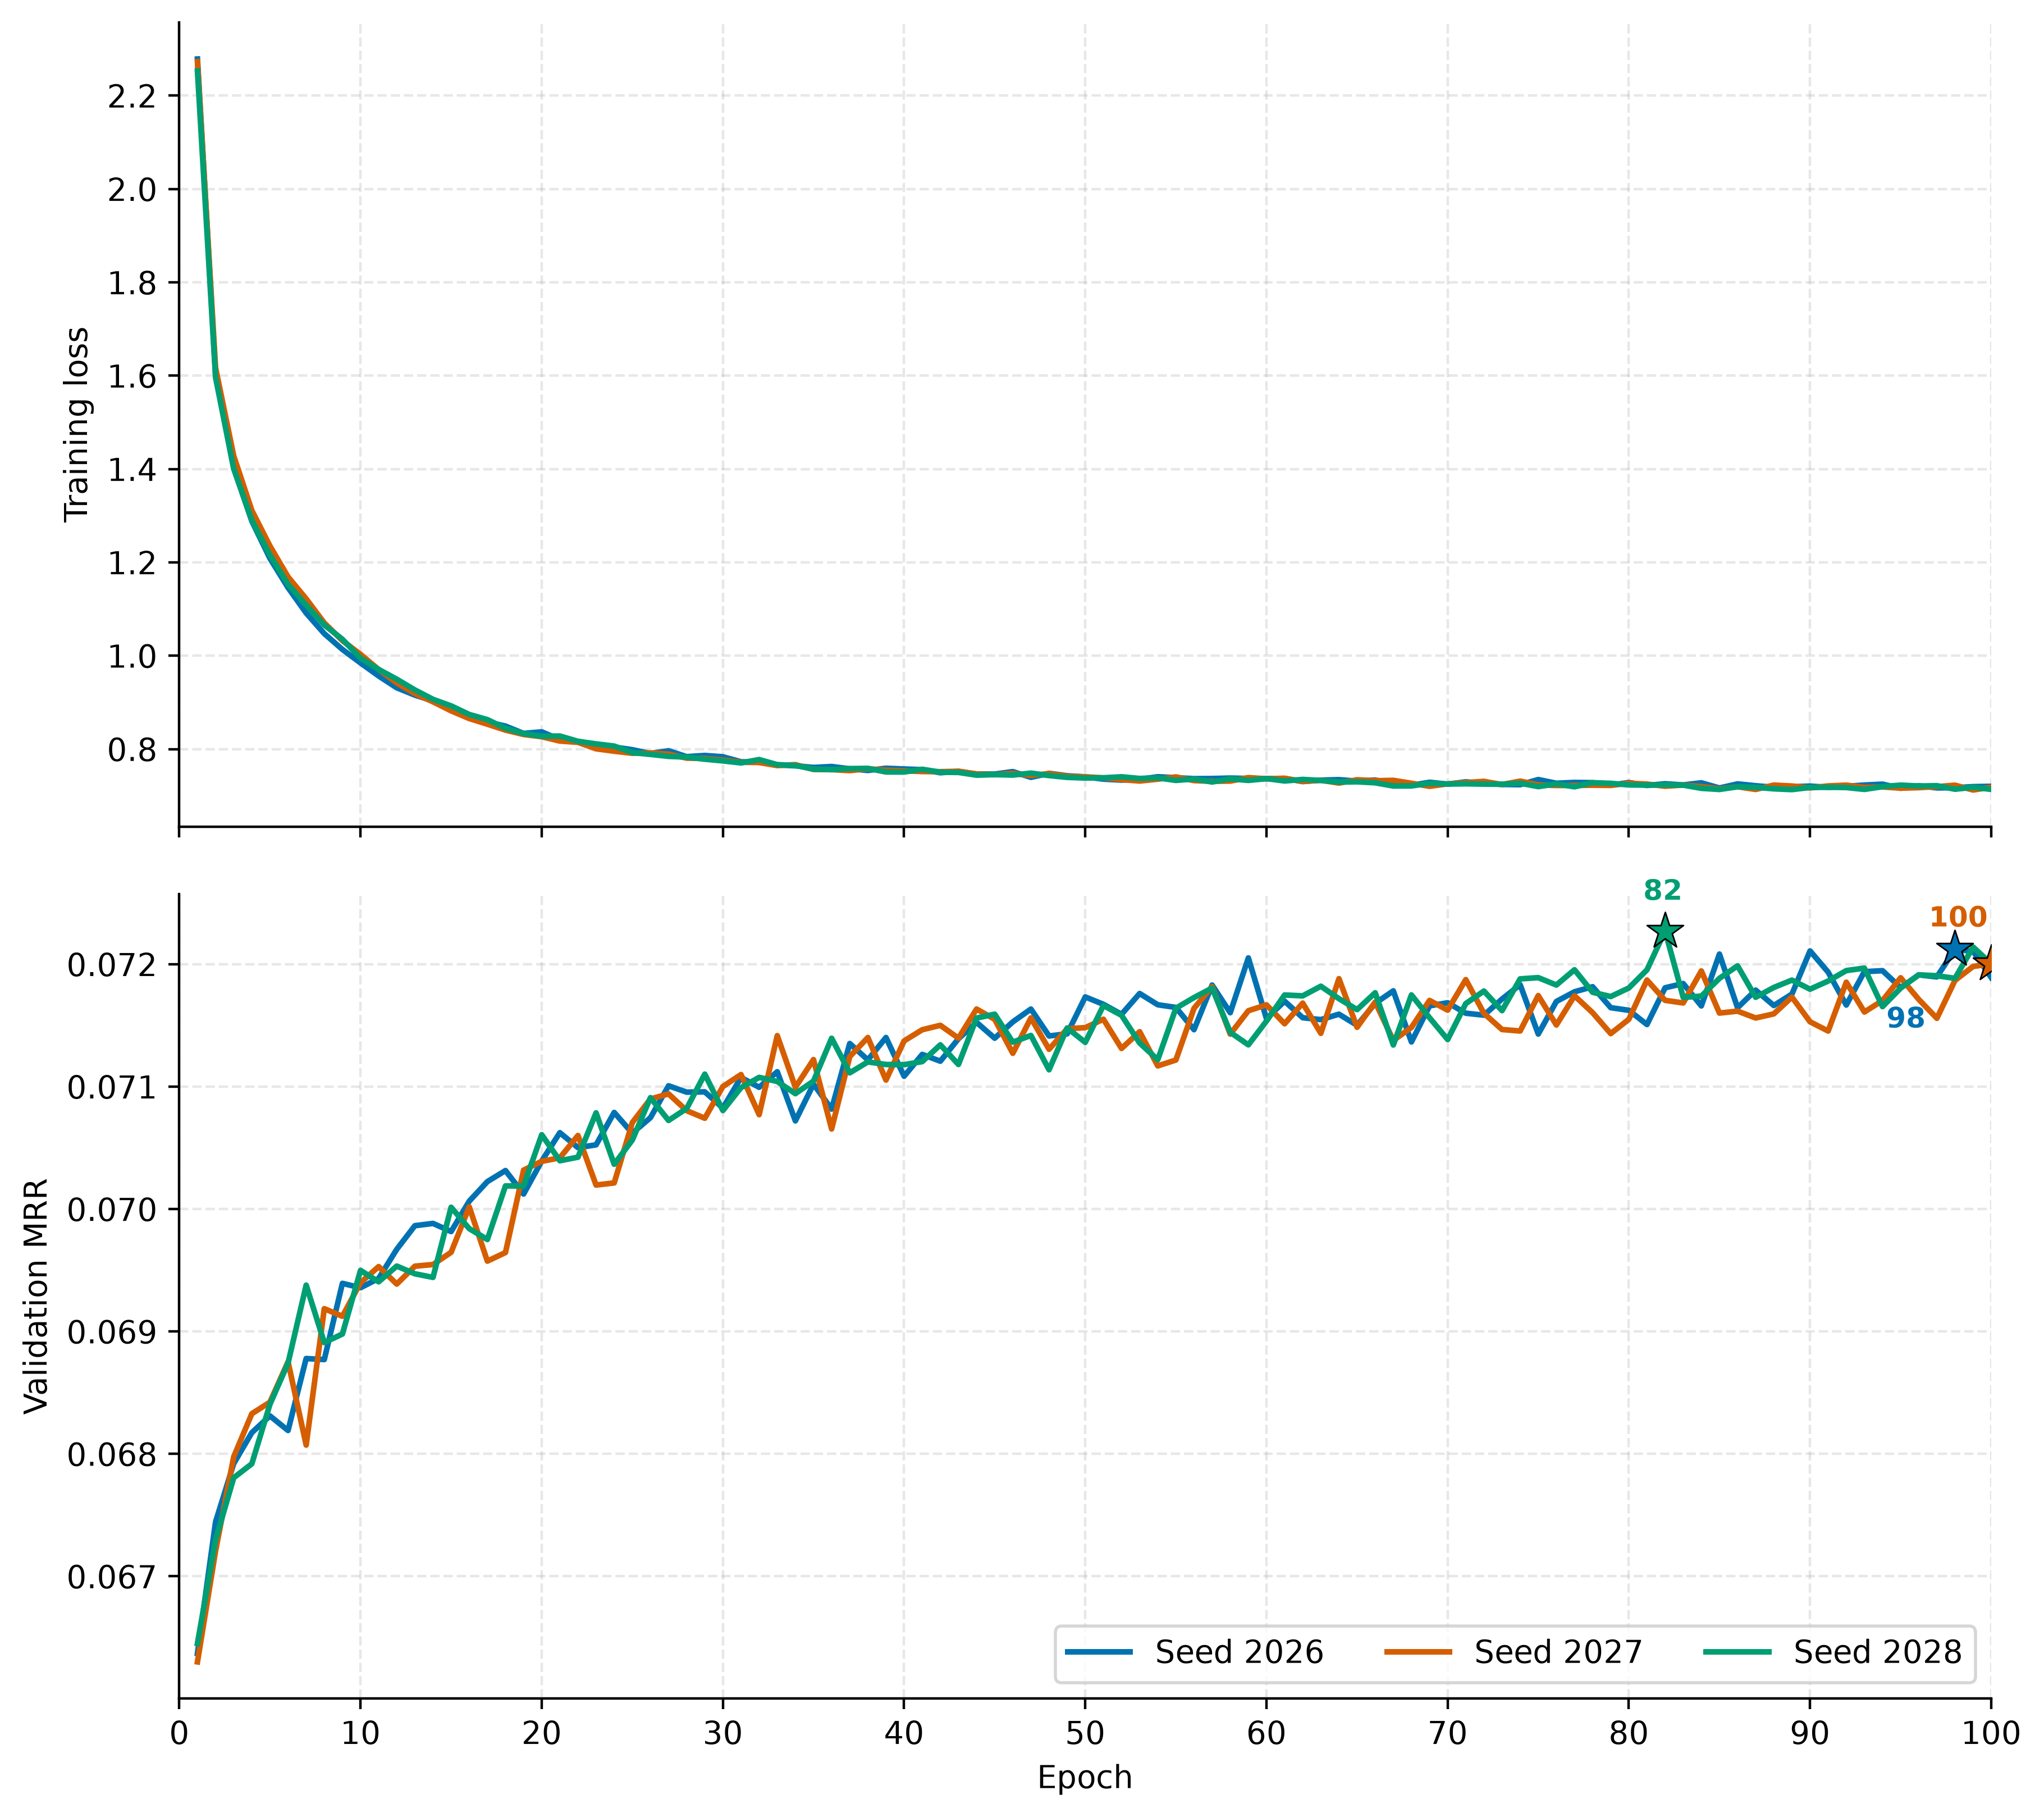
\includegraphics[width=\columnwidth]{figures/visual_genome_convergence.png}
\caption{Training loss và validation MRR trên Visual Genome}
\label{fig:vg-convergence}
\end{figure}

\subsection{So sánh các cấu hình ablation}

\begin{table*}[!t]
\centering
\footnotesize
\setlength{\tabcolsep}{4pt}
\caption{So sánh các cấu hình trên Visual Genome (mỗi cấu hình một lần huấn luyện)}
\label{tab:vg-ablation}
\begin{tabular}{lrrrrrr}
\toprule
Cấu hình & Epoch & $\alpha_{\mathrm{CLIP}}$ & R@1 & R@5 & R@10 & MRR\\
\midrule
CLIP-only &  & 1.0 & 0.0295 & 0.0793 & 0.1165 & 0.0611\\
No-edge & 85 & 0.6 & 0.0346 & 0.0921 & 0.1333 & 0.0692\\
Random-edges & 99 & 0.6 & 0.0356 & 0.0943 & 0.1365 & 0.0708\\
Full Graph & 98 & 0.6 & \textbf{0.0361} & \textbf{0.0960} & \textbf{0.1380} & \textbf{0.0717}\\
\bottomrule
\end{tabular}
\end{table*}

Bảng~\ref{tab:vg-ablation} so sánh bốn cấu hình, mỗi cấu hình một lần huấn luyện với cùng khởi tạo. Thứ tự Full Graph, Random-edges, No-edge, CLIP-only giữ trên cả bốn chỉ số. No-edge, không truyền tin giữa các đỉnh, đã tăng MRR khoảng 13\% so với CLIP-only, tức giữ khoảng 77\% mức tăng của Full Graph; phần này đến từ lớp chiếu và cơ chế kết hợp điểm được huấn luyện. Random-edges, hoán vị đỉnh đích nhưng giữ bậc, giữ khoảng 92\%. Full Graph chỉ cao hơn Random-edges khoảng 1.2\% MRR. Như vậy CLIP + GAT cải thiện rõ so với CLIP, nhưng phần lớn lợi ích không đến từ việc biểu diễn đúng quan hệ giữa các thực thể; kết luận này mới dựa trên một lần chạy ablation.


\subsection{Giải thích kết quả xếp hạng}
\label{sec:level1-xai-results}

Bộ giải thích ở Mục~\ref{sec:level1-xai-method} được chạy trên cả ba checkpoint của Full Graph. $K^\star = 12$ được chọn trên validation là $K$ nhỏ nhất có trung vị độ đầy đủ từ 0.8 trở lên. Tính lại điểm đồ thị từ đồ thị gốc cho toàn bộ 523\,347 truy vấn test khớp kết quả đã lưu của checkpoint chính (MRR 0.0717, sai khác $3 \times 10^{-7}$), nên giải thích được đo trên đúng mô hình đã báo cáo. Trên 500 truy vấn test, bỏ các quan hệ trong giải thích làm xác suất của ảnh trả về giảm $\text{Fid}^{+} = 0.118 \pm 0.002$. Bỏ cùng số quan hệ ngẫu nhiên chỉ cho 0.003, hiệu số 0.114 (CI 95\% $[0.110, 0.118]$). Tập giải thích có trung bình 11.1 quan hệ. Bỏ cùng số quan hệ có attention lớn nhất cho $-0.007$, tức trọng số attention không chỉ ra quan hệ quyết định điểm. PN là 0.357 so với 0.053 khi chọn ngẫu nhiên. Chỉ giữ tập giải thích cho ảnh điểm cao hơn cả đồ thị đầy đủ ($\text{Fid}^{-}$ trung vị $-0.193$, PS 1.000). 75\% phần tử của giải thích là cạnh \texttt{contains} từ đỉnh ảnh. 24.2\% phần tử chạm một vật có tên trùng từ trong câu truy vấn, so với 18.4\% với cùng số phần tử ngẫu nhiên ($p \approx 10^{-25}$).

Trong 20\,000 truy vấn test bốc ngẫu nhiên, 5\,243 truy vấn có ảnh đúng nằm trong top-50 CLIP. Trong số này, CLIP + GAT đưa 247 truy vấn từ hạng lớn hơn 1 lên hạng 1; No-edge cũng làm được với 153 truy vấn, và chỉ 54 truy vấn cần đồ thị thật (cả No-edge lẫn Random-edges đều không đạt hạng 1). Ngược lại, 114 truy vấn CLIP xếp đúng ở hạng 1 bị CLIP + GAT đẩy xuống. Con số này khớp với ablation: phần lớn lợi ích đến từ phép chiếu đặc trưng của chính ảnh; trong phần do đồ thị, giải thích chủ yếu chỉ ra các vật có trong ảnh hơn là quan hệ giữa chúng.

\textbf{Năm ca thành công và năm ca thất bại.} Ca được chọn theo luật cố định trên 20\,000 truy vấn test: thành công khi CLIP xếp ảnh đúng ở hạng lớn hơn 1, CLIP + GAT xếp hạng 1, đồng thời cả No-edge và Random-edges đều xếp hạng lớn hơn 1, để thành công có thể quy cho quan hệ thật; thất bại gồm 3 ca đồ thị làm hại (CLIP hạng 1, CLIP + GAT tụt hạng) và 2 ca không cứu được (CLIP + GAT ở hạng 2 đến 5). Bảng~\ref{tab:vg-cases} tóm tắt 10 ca.

\begin{table*}[!t]
\centering
\footnotesize
\setlength{\tabcolsep}{3.5pt}
\caption{Năm ca thành công và năm ca thất bại trên Visual Genome: hạng của ảnh đúng theo từng cấu hình và sau khi bỏ tập giải thích $S$ ($K^\star = 12$)}
\label{tab:vg-cases}
\begin{tabularx}{\textwidth}{lYrrrrrY}
\toprule
Loại & Truy vấn & CLIP & \twoline{CLIP +}{GAT} & No-edge & Random & Bỏ $S$ & Phần tử đóng góp lớn nhất ($\Delta \times 10^{-3}$)\\
\midrule
Thành công & Guy holding up peace sign & 15 & 1 & 4 & 2 & 4 & ảnh chứa peace sign $\times$5 (5.5 mỗi cạnh)\\
Thành công & Yellow flowers in a purple and yellow rain boot & 14 & 1 & 2 & 3 & 4 & ảnh chứa rain boots (2.6)\\
Thành công & biohazard sign placed on bathroom medicine cabinet & 11 & 1 & 2 & 6 & 1 & ảnh chứa bathroom (2.6)\\
Thành công & brown suitcase in airport & 11 & 1 & 5 & 4 & 2 & ảnh chứa green suitcase (2.0)\\
Thành công & a man holding a umbrella & 10 & 1 & 3 & 2 & 4 & ảnh chứa rain (2.0), umbrella (1.4)\\
\midrule
Làm hại & large black train & 1 & 3 & 1 & 2 & 3 & ảnh chứa steam (0.9), people $\times$5\\
Làm hại & A man on the road & 1 & 3 & 1 & 1 & 7 & ảnh chứa road (3.2), man (2.8)\\
Làm hại & a slice of spinach and cheese pizza & 1 & 3 & 3 & 2 & 3 & ảnh chứa spinach $\times$4 (0.8 mỗi cạnh)\\
Không cứu & pink beak on bird & 2 & 5 & 5 & 5 & 8 & ảnh chứa bird (1.2), beak (1.0)\\
Không cứu & woman wearing green shorts & 10 & 3 & 1 & 1 & 4 & ảnh chứa shorts $\times$2 (3.9 mỗi cạnh)\\
\bottomrule
\end{tabularx}
\end{table*}

\textbf{Thành công.} Trong cả 5 ca, phần tử đóng góp lớn nhất là cạnh \texttt{contains} tới vật được nhắc trong truy vấn (peace sign, rain boots, suitcase, umbrella). Ở 4 ca, bỏ tập giải thích làm ảnh đúng rơi xuống hạng 2 đến 4, nên giải thích đúng là phần đưa ảnh lên hạng 1. Quan hệ giữa hai vật có xuất hiện trong giải thích nhưng đóng góp nhỏ hơn 7 đến 26 lần so với phần tử lớn nhất: trong ca ``Guy holding up peace sign'', \textit{man holding up peace sign} chỉ đạt $0.2 \times 10^{-3}$ so với $5.5 \times 10^{-3}$ của mỗi cạnh \textit{ảnh chứa peace sign} (Hình~\ref{fig:vg-case}). Ca ``biohazard sign'' là ngoại lệ: bỏ mọi cạnh của ảnh hầu như không đổi điểm đồ thị và bỏ $S$ vẫn giữ hạng 1, nên thứ hạng ở đây đến từ biểu diễn của chính đỉnh ảnh qua mô hình đầy đủ, không từ các vật hay quan hệ.

\textbf{Thất bại.} Ba ca làm hại có chung một cơ chế. Ảnh sai ở hạng 1 cũng chứa các vật khớp với truy vấn (train, road và man, spinach) và được giải thích bằng chính các cạnh \texttt{contains} đó. Mô hình thưởng cho sự có mặt của vật nhưng không phân biệt được thuộc tính (\textit{black}, \textit{slice}) hay quan hệ không gian (\textit{on the road}). Ở ca pizza, cạnh \textit{ảnh chứa spinach} của ảnh sai có $\Delta = 1.4 \times 10^{-3}$, cao hơn $0.8 \times 10^{-3}$ của ảnh đúng. Ca ``woman wearing green shorts'' tương tự: ảnh sai có \textit{ảnh chứa shorts} với $\Delta = 14.9 \times 10^{-3}$, còn quan hệ \textit{woman wearing shorts} của ảnh đúng chỉ đạt $0.1 \times 10^{-3}$. Ở 3 trên 5 ca thất bại, No-edge vẫn xếp ảnh đúng hạng 1, nên lỗi xuất hiện khi thêm bước truyền tin qua các cạnh của scene graph. Chú thích cảnh của Visual Genome còn có quan hệ nhiễu (\textit{no u turn saying no u turn}) và tên vật trùng lặp, làm giải thích dài hơn cần thiết.

\begin{figure*}[!t]
\centering
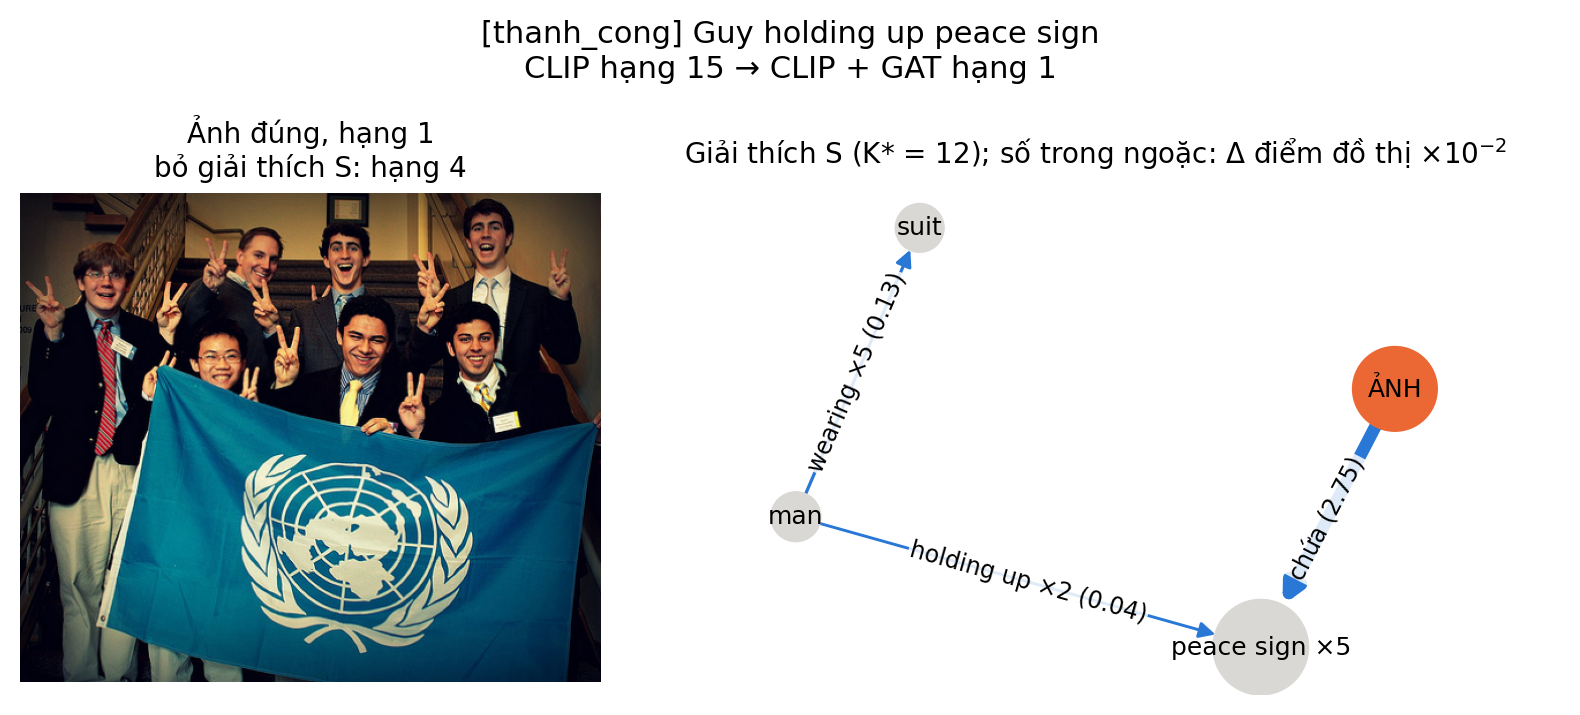
\includegraphics[width=0.8\textwidth]{figures/case_vg_success_peacesign.png}
\caption{Ca thành công ``Guy holding up peace sign'' trên Visual Genome: CLIP hạng 15, CLIP + GAT hạng 1, bỏ tập giải thích thì ảnh về hạng 4. Đồ thị vẽ đúng tập giải thích $S$ ($K^\star = 12$); nút cam là đỉnh ảnh, nút và quan hệ cùng tên được gộp ($\times n$). Độ dày cạnh và số trong ngoặc là tổng mức giảm điểm đồ thị khi bỏ các quan hệ đó ($\Delta$, đơn vị $10^{-2}$).}
\label{fig:vg-case}
\end{figure*}

\section{Cấp độ 2: Truy vấn trên đồ thị tri thức đa phương thức}
\label{sec:level2-results}

\subsection{Hiệu năng trên DB15K và FB15K-237-IMG}

Checkpoint và $\alpha_{\mathrm{CLIP}}$ được chọn trên validation: $\alpha_{\mathrm{CLIP}}$ là 0.0 hoặc 0.1 trên DB15K và 0.1 trên FB15K-237-IMG. Khi $\alpha_{\mathrm{CLIP}} = 0$, CLIP vẫn quyết định tập top-1\,000 và thứ tự ngoài tập này. Bảng~\ref{tab:level2-main} so sánh CLIP với AdaMF và với GAT cấp 1 chạy trên cùng pipeline DB15K (Mục~\ref{sec:level2-gat}).

\begin{table}[!t]
\centering
\footnotesize
\setlength{\tabcolsep}{1.8pt}
\caption{Kết quả test trên DB15K và FB15K-237-IMG (trung bình ba lần huấn luyện, độ lệch chuẩn không quá 0.004 ở mọi ô; R@K tính trên mọi truy vấn)}
\label{tab:level2-main}
\begin{tabular}{lrrrrrr}
\toprule
 & & & & \multicolumn{3}{c}{MRR}\\
\cmidrule(l){5-7}
Mô hình & R@1 & R@5 & R@10 & Gộp & \twoline{Trực}{tiếp} & \twoline{Gián}{tiếp}\\
\midrule
\multicolumn{7}{l}{\textit{DB15K}}\\
CLIP & 0.2123 & 0.3002 & 0.3412 & 0.2577 & 0.5520 & 0.0475\\
CLIP + AdaMF & \textbf{0.3395} & 0.4955 & \textbf{0.5519} & \textbf{0.4133} & 0.5520 & \textbf{0.3143}\\
CLIP + GAT & 0.3368 & \textbf{0.4967} & 0.5491 & 0.4114 & 0.5520 & 0.3110\\
\midrule
\multicolumn{7}{l}{\textit{FB15K-237-IMG}}\\
CLIP & 0.0760 & 0.1181 & 0.1394 & 0.0991 & 0.3475 & 0.0122\\
CLIP + AdaMF & \textbf{0.2581} & \textbf{0.3214} & \textbf{0.3492} & \textbf{0.2892} & \textbf{0.7770} & \textbf{0.1186}\\
\bottomrule
\end{tabular}
\end{table}

Trên DB15K, truy vấn trực tiếp giữ thứ hạng CLIP theo thiết kế, nên toàn bộ mức tăng nằm ở nhóm gián tiếp: MRR gián tiếp tăng từ 0.0475 lên 0.3143, gấp 6.6 lần; nhóm tail (0.0699 lên 0.4714) tăng mạnh hơn nhóm head (0.0303 lên 0.1933). Trên FB15K-237-IMG, mô hình xếp hạng lại cả hai nhóm; MRR trực tiếp tăng từ 0.3475 lên 0.7770 và gián tiếp từ 0.0122 lên 0.1186. Độ lệch chuẩn giữa các lần huấn luyện nhỏ hơn 0.003 ở mọi chỉ số.

\textbf{GAT so với AdaMF trên cùng pipeline.} Trên validation, MRR gián tiếp của GAT thấp hơn AdaMF 0.0037 với khoảng tin cậy bootstrap 95\% là $[-0.0076, +0.0005]$, tức hai phương pháp không phân biệt được; theo quy tắc chọn trước, AdaMF được giữ làm phương pháp chính cho cấp 3. Trên test (chỉ báo cáo), hiệu số là $-0.0033$, CI 95\% $[-0.0070, +0.0005]$, Wilcoxon $p = 0.055$. Như vậy trên DB15K, phần lớn lợi ích đến từ việc học nhúng thực thể từ cấu trúc đồ thị và bộ chấm RotatE, không riêng cơ chế dung hợp của AdaMF.

\subsection{Đối chứng cấu trúc đồ thị}
\label{sec:level2-graph-ablation}

Mỗi đối chứng được huấn luyện một lần, chọn checkpoint và $\alpha_{\mathrm{CLIP}}$ riêng trên validation (Bảng~\ref{tab:level2-ablation}). Đồ thị xáo cạnh trên DB15K có 71\,300 cạnh và không trùng bộ ba validation/test.

\begin{table}[!t]
\centering
\footnotesize
\setlength{\tabcolsep}{4pt}
\caption{Ablation cấu trúc đồ thị (MRR test, mỗi biến thể một lần huấn luyện)}
\label{tab:level2-ablation}
\begin{tabular}{lrrrr}
\toprule
Cấu hình & $\alpha_{\mathrm{CLIP}}$ & Gộp & Gián tiếp & Giữ lại\\
\midrule
\multicolumn{5}{l}{\textit{DB15K}}\\
Đồ thị gốc & 0.0 & 0.4145 & 0.3164 & 100\%\\
Xáo cạnh & 0.2 & 0.3156 & 0.1468 & 37\%\\
Đồ thị ngẫu nhiên & 1.0 & 0.2577 & 0.0475 & 0\%\\
Bỏ cạnh & 1.0 & 0.2577 & 0.0475 & 0\%\\
\midrule
\multicolumn{5}{l}{\textit{FB15K-237-IMG}}\\
Đồ thị gốc & 0.1 & 0.2896 & 0.1198 & 100\%\\
Xáo cạnh & 0.1 & 0.2879 & 0.1121 & 93\%\\
Đồ thị ngẫu nhiên & 0.1 & 0.2869 & 0.1121 & 93\%\\
Bỏ cạnh & 1.0 & 0.0991 & 0.0122 & 0\%\\
\bottomrule
\end{tabular}
\par\smallskip{\footnotesize Giữ lại: phần mức tăng MRR gián tiếp so với CLIP còn lại, (biến thể $-$ CLIP) / (đồ thị gốc $-$ CLIP).}
\end{table}

Trên DB15K, khi bỏ cạnh hoặc dùng đồ thị ngẫu nhiên, validation chọn $\alpha_{\mathrm{CLIP}} = 1$, tức điểm đồ thị không còn giúp gì; xáo cạnh (giữ bậc theo quan hệ) chỉ giữ 37\% mức tăng gián tiếp. Phần lớn cải thiện cần đúng cạnh thật. Trên FB15K-237-IMG, kết luận ngược lại: xáo cạnh và đồ thị ngẫu nhiên vẫn giữ khoảng 93\% mức tăng gián tiếp và toàn bộ mức tăng trực tiếp. Pipeline FB15K-237-IMG học bằng mục tiêu truy hồi trên truy vấn huấn luyện; ablation đổi thực thể neo nhưng giữ ảnh đích, nên mô hình vẫn học được thực thể nào khớp với ảnh nào. Vì vậy trên FB15K-237-IMG không chứng minh được mức tăng đến từ cấu trúc quan hệ; DB15K là bằng chứng chính ở cấp 2. Ablation mới chạy một lần.

\subsection{Bộ 20 truy vấn đánh giá}
\label{sec:level2-benchmark}

Mỗi tập có 20 truy vấn (10 trực tiếp, 5 head, 5 tail) chọn theo luật cố định trước khi xem kết quả: lấy từ test, bỏ truy vấn có thực thể đích không xuất hiện trong train, mỗi thực thể đích một truy vấn, bốc ngẫu nhiên cố định. Bộ này chỉ dùng để đánh giá và minh họa giải thích. Truy vấn gián tiếp có dạng ``tìm ảnh của thực thể có quan hệ \textit{r} với \textit{anchor}'', ví dụ ``\textit{an image of the entity that is related to Angelina Jolie by spouse}''.

\begin{table}[!t]
\centering
\footnotesize
\setlength{\tabcolsep}{4pt}
\caption{MRR trên bộ 20 truy vấn (AdaMF: trung bình các lần huấn luyện)}
\label{tab:level2-benchmark}
\begin{tabular}{lrr}
\toprule
Nhóm (n) & CLIP & CLIP + AdaMF\\
\midrule
\multicolumn{3}{l}{\textit{DB15K}}\\
Trực tiếp (10) & 0.306 & 0.306\\
Gián tiếp (10) & 0.003 & \textbf{0.296}\\
Tất cả (20) & 0.154 & \textbf{0.301}\\
\midrule
\multicolumn{3}{l}{\textit{FB15K-237-IMG}}\\
Trực tiếp (10) & 0.410 & \textbf{0.878}\\
Gián tiếp (10) & 0.012 & 0.025\\
Tất cả (20) & 0.211 & \textbf{0.451}\\
\bottomrule
\end{tabular}
\end{table}

Trên DB15K, 4 trong 10 truy vấn gián tiếp được đưa từ hạng vài trăm của CLIP lên top 5 ở mọi lần huấn luyện, ví dụ truy vấn về vợ, chồng của Angelina Jolie từ hạng 363 lên 2 và người kế nhiệm Robert Byrd từ hạng 242 lên 1. Trên FB15K-237-IMG, mức tăng gần như chỉ ở nhóm trực tiếp, khớp với kết quả ablation. Mười truy vấn mỗi nhóm quá ít để kiểm định; kết quả trên toàn bộ tập test ở Bảng~\ref{tab:level2-main} là bằng chứng chính.

\subsection{Giải thích và phân tích ca}
\label{sec:level2-cases}

Mỗi ảnh được giải thích theo ba tầng: thực thể quyết định (thực thể đạt điểm cao nhất trong số thực thể gắn với ảnh), đóng góp của từng phương thức (đo bằng che phương thức) và $K^\star$ bộ ba train có đóng góp lớn nhất ($K^\star = 2$ trên DB15K, 8 trên FB15K-237-IMG). Hình~\ref{fig:case-db15k} là một ca thành công trên DB15K.

\begin{figure*}[!t]
\centering
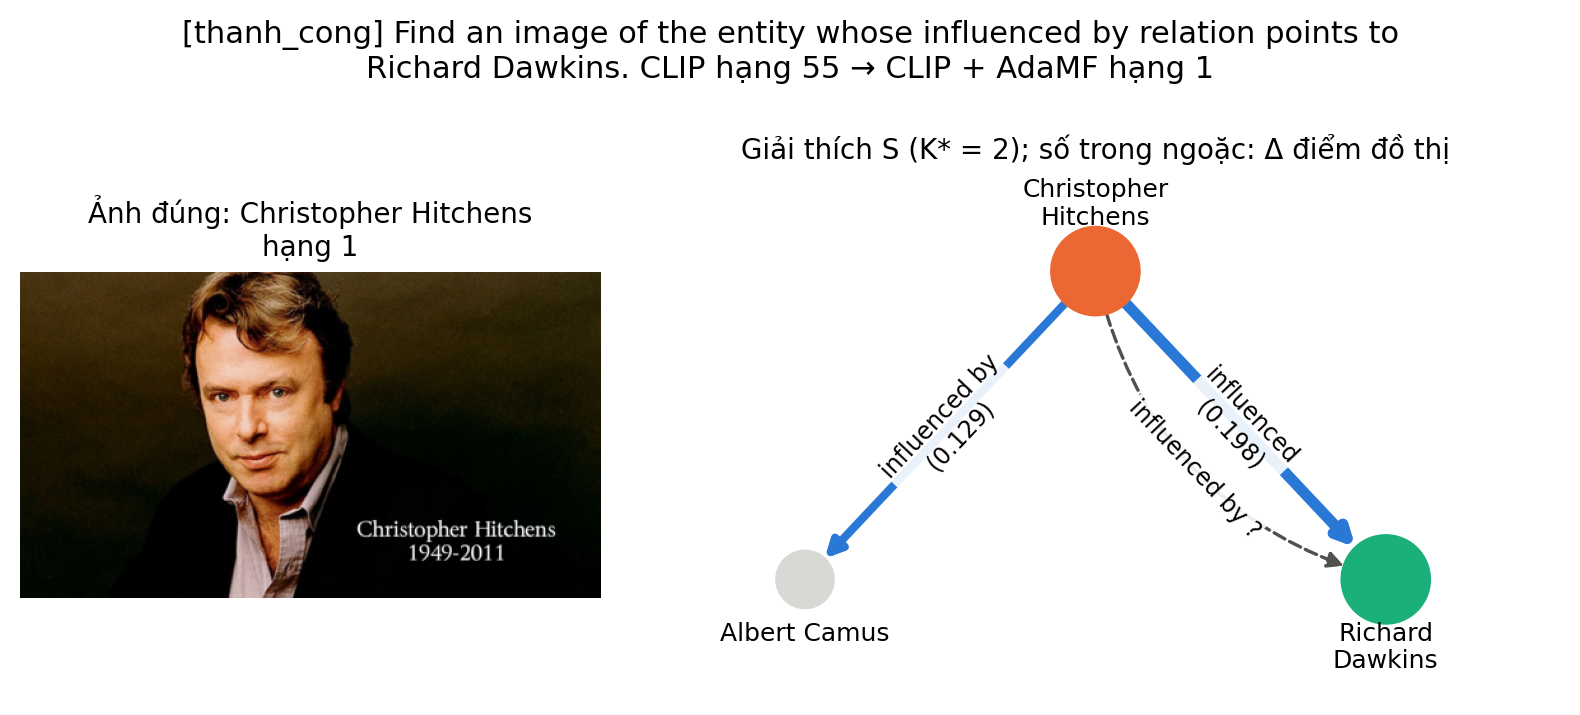
\includegraphics[width=0.78\textwidth]{figures/case_db15k_success_hitchens.png}
\caption{Ca thành công trên DB15K: truy vấn tìm thực thể có quan hệ \textit{influenced by} tới Richard Dawkins (nút xanh ngọc, ảnh trả về là nút cam); CLIP xếp ảnh đúng ở hạng 55, CLIP + AdaMF ở hạng 1. Đồ thị: hai bộ ba giải thích ($K^\star = 2$, nét liền, độ dày và số trong ngoặc là $\Delta$), trong đó Christopher Hitchens \textit{influenced} Richard Dawkins ($\Delta = 0.198$) nối trực tiếp với thực thể neo; nét đứt là quan hệ được hỏi. Che từng phương thức: điểm đồ thị giảm 74.8 khi che cấu trúc, $-0.15$ khi che ảnh và 0.20 khi che văn bản.}
\label{fig:case-db15k}
\end{figure*}

\textbf{DB15K.} Năm ca thành công đều đưa ảnh đúng từ hạng 55 đến 624 của CLIP lên hạng 1; ba ca có bộ ba giải thích là đường đi một bước từ thực thể neo, ví dụ Timbaland \textit{associated musical artist} Missy Elliot ($\Delta = +0.335$). Bỏ hai bộ ba giải thích làm điểm đồ thị giảm 0.32 đến 2.0, so với $-0.05$ đến 0.56 khi bỏ hai bộ ba ngẫu nhiên. Năm ca thất bại cho thấy ba nguyên nhân: (1) hai ứng viên cùng được nối với thực thể neo bằng một quan hệ gần nghĩa, như Rock Hudson \textit{known for} cả Pillow Talk lẫn Dynasty cho truy vấn \textit{starring}, hay Soul jazz và Funk cùng có \textit{stylistic origin} Soul music; (2) bằng chứng là bộ ba nhiễu của dữ liệu như Maurice Sendak \textit{type} Island; (3) mô hình trả về chính thực thể neo (Arthur C. Clarke cho truy vấn ``chịu ảnh hưởng bởi Arthur C. Clarke'').

\textbf{FB15K-237-IMG.} Thực thể quyết định của các ca thành công thường là thực thể trung tâm có hàng nghìn bộ ba (United States of America, English Language, New York City); mỗi bộ ba chỉ đóng góp khoảng $10^{-4}$, và che phương thức văn bản đôi khi làm điểm giảm nhiều như che phương thức cấu trúc. Điều này phù hợp với kết quả ablation: trên FB15K-237-IMG, mô hình dựa ít vào từng quan hệ cụ thể.

\section{Cấp độ 3: Giải thích định lượng và chuyển giao sang ViHeritage-MMKG}
\label{sec:level3-results}

\subsection{Truy vấn trên ViHeritage-MMKG}
\label{sec:level3-custom-mmkg}

\begin{table}[!t]
\centering
\footnotesize
\setlength{\tabcolsep}{2pt}
\caption{Kết quả test trên ViHeritage-MMKG, câu tiếng Việt (trung bình $\pm$ độ lệch chuẩn mẫu; R@K tính trên cả 142 truy vấn; 88 truy vấn trực tiếp giữ thứ hạng CLIP, MRR 0.156)}
\label{tab:viheritage-results}
\begin{tabular}{lrrrrr}
\toprule
 & & & & \multicolumn{2}{c}{MRR}\\
\cmidrule(l){5-6}
Mô hình & R@1 & R@5 & R@10 & \twoline{Gộp}{(142)} & \twoline{Gián tiếp}{(54)}\\
\midrule
CLIP & 0.053 & 0.183 & 0.324 & 0.139 & 0.112\\
CLIP + AdaMF & 0.069 & 0.248 & 0.430 & 0.180\pmsd{0.004} & 0.219\pmsd{0.012}\\
CLIP + GAT & \textbf{0.080} & \textbf{0.282} & \textbf{0.465} & \textbf{0.195}\pmsd{0.014} & \textbf{0.258}\pmsd{0.036}\\
\bottomrule
\end{tabular}
\end{table}

Bảng~\ref{tab:viheritage-results} cho thấy đồ thị giúp rõ ở truy vấn gián tiếp: so với CLIP, MRR tăng 0.107 với AdaMF (CI 95\% $[0.030, 0.185]$, Wilcoxon $p = 0.006$, 36 truy vấn tốt hơn và 18 kém hơn) và 0.146 với GAT (CI 95\% $[0.065, 0.230]$, $p = 0.0007$). Hiệu số GAT trừ AdaMF là 0.039, CI 95\% $[-0.008, 0.089]$, $p = 0.29$, nên hai mô hình không phân biệt được trên test. Với câu tiếng Anh, MRR gián tiếp là 0.248 (AdaMF) và 0.266 (GAT) so với 0.138 của CLIP. Theo quan hệ, mức tăng lớn nhất ở \textit{thuộc quần thể}, \textit{danh hiệu di sản}, \textit{tôn giáo} và \textit{nằm ở tỉnh}; ngược lại, với \textit{là một} và \textit{xây dựng vào thế kỷ}, điểm đồ thị làm kết quả kém hơn CLIP.

\textbf{Ablation.} Với một lần huấn luyện mỗi biến thể, bỏ cạnh làm validation chọn $\alpha_{\mathrm{CLIP}} = 1$ (AdaMF) và 0.9 (GAT), MRR gián tiếp quay về mức CLIP; xáo cạnh cho 0.079 (AdaMF) và 0.107 (GAT), thấp hơn cả CLIP. MRR hoàn thiện đồ thị trên bộ ba test giảm từ khoảng 0.33 xuống 0.03 khi bỏ cạnh và 0.17 đến 0.19 khi xáo cạnh. Khác với Visual Genome và FB15K-237-IMG, trên ViHeritage toàn bộ lợi ích phụ thuộc vào đúng cạnh thật.

\textbf{Chuyển giao.} Lợi ích ở truy vấn gián tiếp giảm từ 6.6 lần trên DB15K xuống 1.95 lần (AdaMF) và 2.30 lần (GAT) trên ViHeritage; một nguyên nhân có thể là đồ thị rất nhỏ (318 bộ ba train). Thứ tự hai phương pháp giữ ở mức không phân biệt được trên cả DB15K và test ViHeritage, dù trên validation ViHeritage GAT tốt hơn (hiệu số 0.057, CI 95\% $[0.007, 0.105]$). Để loại khả năng lợi ích đến từ văn bản rò rỉ (38.9\% truy vấn có tên thực thể neo trong mô tả của đáp án), nhóm huấn luyện lại AdaMF với văn bản bị che hoàn toàn: MRR gián tiếp đạt 0.230, không thấp hơn bản đầy đủ (0.219; hiệu số $-0.011$, CI 95\% $[-0.044, 0.023]$), giữ 110\% lợi ích. Lợi ích của đồ thị vì vậy không đến từ văn bản rò rỉ.

\subsection{Đánh giá giải thích định lượng}
\label{sec:level3-xai}

Bảng~\ref{tab:xai-all} tổng hợp các chỉ số theo cùng định nghĩa cho mọi cấp độ; Hình~\ref{fig:xai-fidelity} và Hình~\ref{fig:xai-kcurve} trực quan hai kết quả chính.

\begin{table*}[!t]
\centering
\footnotesize
\setlength{\tabcolsep}{3pt}
\caption{Đánh giá giải thích tại $K^\star$ (trung bình $\pm$ độ lệch chuẩn giữa các lần huấn luyện; $\text{Fid}^{-}$ và Fid làm nhiễu là trung vị trong mỗi lần)}
\label{tab:xai-all}
\begin{tabular}{llrrrrrrrrrr}
\toprule
Dữ liệu, mô hình & Bộ giải thích & $K^\star$ & Fid+ & \twoline{Fid+}{ngẫu nhiên} & \twoline{Fid làm}{nhiễu} & Fid$-$ & PN & \twoline{PN}{ngẫu nhiên} & PS & Sparsity & Ổn định\\
\midrule
Visual Genome, GAT & Bỏ quan hệ & 12 & 0.118\pmsd{0.002} & 0.003 & 0.063 & $-$0.193 & 0.357 & 0.053 & 1.000 & 0.647 & 0.552\\
DB15K, AdaMF & Học lại nhúng & 2 & 0.511\pmsd{0.065} & 0.023 & 0.431 & $-$0.905 & 0.643 & 0.230 & 0.681 & 0.799 & 0.625\\
FB15K-237-IMG, AdaMF & Học lại nhúng & 8 & 0.335\pmsd{0.041} & 0.011 & 0.043 & $-$0.938 & 0.757 & 0.248 & 0.976 & 0.795 & 0.421\\
ViHeritage, AdaMF & Học lại nhúng & 1 & 0.535\pmsd{0.059} & 0.145 & 0.059 & 0.861 & 0.773 & 0.401 & 0.144 & 0.786 & 0.396\\
ViHeritage, GAT & Che cạnh & 8 & 0.103\pmsd{0.080} & 0.002 & 0.024 & $-$0.112 & 0.370 & 0.072 & 0.981 & 0.762 & 0.364\\
\bottomrule
\end{tabular}
\par\smallskip{\footnotesize Cấp 1: Visual Genome; cấp 2: DB15K, FB15K-237-IMG; cấp 3: ViHeritage. Ổn định: Jaccard trung bình của tập giải thích giữa các cặp mô hình huấn luyện độc lập khi chúng trả về cùng ảnh. Validity cấu trúc đạt 100\% ở mọi dòng: với Visual Genome, mọi phần tử là quan hệ có trong scene graph của chính ảnh và nằm trong vùng tiếp nhận hai bước; với các tập còn lại, mọi phần tử là bộ ba train, không trùng validation/test. Số truy vấn: Visual Genome 500, DB15K và FB15K-237-IMG 70, ViHeritage 54 với GAT và 50 với AdaMF.}
\end{table*}

\begin{figure}[!t]
\centering
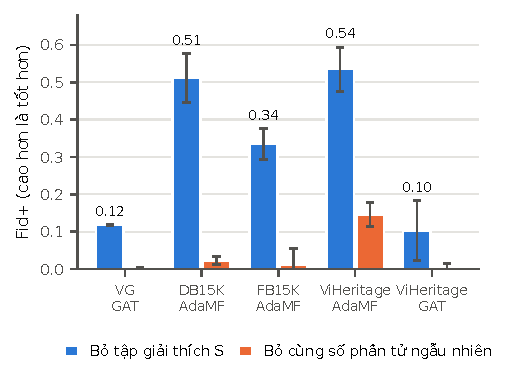
\includegraphics[width=\columnwidth]{figures/fig_xai_fidelity.pdf}
\caption{Fid+ khi bỏ tập giải thích so với bỏ cùng số phần tử ngẫu nhiên (trung bình $\pm$ độ lệch chuẩn giữa các lần huấn luyện). VG: Visual Genome; FB15K: FB15K-237-IMG.}
\label{fig:xai-fidelity}
\end{figure}

\textbf{Fidelity.} Ở mọi mô hình, bỏ đúng tập giải thích làm xác suất của ảnh trả về giảm nhiều hơn hẳn bỏ cùng số phần tử ngẫu nhiên. Trên ViHeritage (54 truy vấn với GAT, 50 với AdaMF), hiệu số Fid+ so với ngẫu nhiên là 0.39 (CI 95\% $[0.35, 0.44]$, $p < 10^{-10}$) với AdaMF và 0.10 ($[0.06, 0.14]$, $p < 10^{-4}$) với GAT; PN cao hơn ngẫu nhiên 0.38 và 0.30. Làm nhiễu, tức thay đầu kia của mỗi phần tử trong $\mathcal{S}$ bằng một thực thể ngẫu nhiên cùng vai trò, cũng làm xác suất của ảnh trả về giảm ở mọi mô hình (trung vị 0.024 đến 0.431, cao nhất trên DB15K), nên kết quả phụ thuộc đúng vào các thực thể mà giải thích chỉ ra. Giải thích cũng tốt hơn heuristic: chọn bộ ba có bậc cao nhất cho Fid+ 0.02 đến 0.21 ở cấp 2 và 3; trên Visual Genome, chọn cùng số quan hệ có attention lớn nhất cho $-0.007$, thấp hơn giải thích 0.125 (CI 95\% $[0.119, 0.131]$). Khi huấn luyện lại AdaMF từ đầu sau khi bỏ bộ ba giải thích, Fid+ là 0.327 so với 0.180 khi bỏ bộ ba ngẫu nhiên ($p = 0.0002$) và 0.197 khi bỏ bộ ba bậc cao ($p = 0.0008$); PN là 0.62 so với 0.52 ($p = 0.075$). Tương quan Spearman giữa Fid+ xấp xỉ và Fid+ khi huấn luyện lại là 0.32, nên phép đo xấp xỉ đúng về hướng nhưng chỉ tương quan vừa phải theo từng truy vấn.

\textbf{Đủ và gọn.} Fid$-$ âm ở Visual Genome, DB15K, FB15K-237-IMG và GAT ViHeritage: chỉ giữ tập giải thích làm ảnh được tin hơn. Riêng AdaMF trên ViHeritage, $K^\star = 1$ cho Fid+ cao nhưng Fid$-$ 0.861 và PS 0.144: một bộ ba là cần thiết nhưng chưa đủ. Hình~\ref{fig:xai-kcurve} cho thấy đánh đổi này; với $K = 2$, Fid$-$ về khoảng 0 và PS tăng lên 0.68 nhưng sparsity giảm từ 0.76 xuống 0.60. Quy tắc chọn $K^\star$ chỉ dựa vào mức giảm điểm khi bỏ, nên ưu tiên tính cần thiết hơn tính đủ. Ngược lại, giải thích của GAT ở cả Visual Genome và ViHeritage có PS cao nhưng Fid+ thấp vì đóng góp phân tán qua nhiều cạnh trong vùng tiếp nhận; trên Visual Genome, Fid+ vẫn tăng khi $K$ vượt $K^\star = 12$ trong khi sparsity giảm còn 0.58 ở $K = 16$.

\begin{figure*}[!t]
\centering
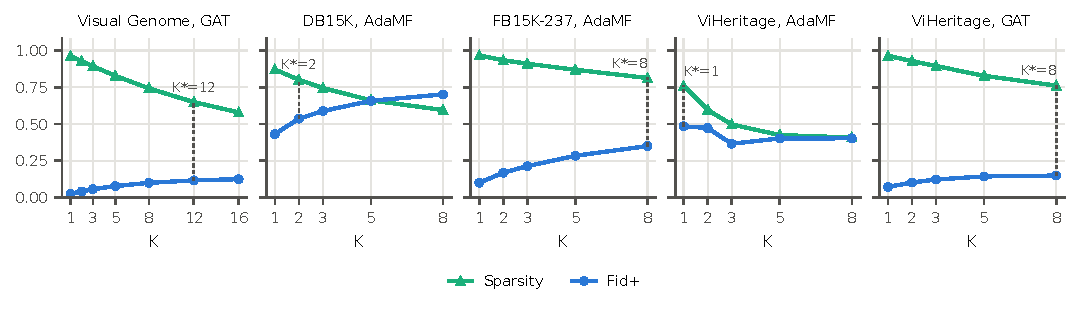
\includegraphics[width=\textwidth]{figures/fig_xai_k_curve.pdf}
\caption{Fid+ và sparsity theo số phần tử $K$ của giải thích (checkpoint chính, test); đường chấm là $K^\star$ chọn trên validation.}
\label{fig:xai-kcurve}
\end{figure*}

\textbf{Validity.} Ở cấp 2 và 3, mọi bộ ba giải thích là bộ ba train và không trùng validation/test; trên Visual Genome, mọi phần tử là quan hệ của chính scene graph của ảnh. Trên ViHeritage, 35\% đến 42\% bộ ba giải thích của AdaMF nằm trên đường đi từ thực thể neo tới thực thể của ảnh; 88\% đến 96\% ảnh trả về của hai mô hình cùng kiểu thực thể với đáp án. Hai mươi ca phân tích (10 mỗi mô hình) được chấm theo kiến thức về di sản, với sự hỗ trợ của công cụ AI, một lượt chấm, không có hệ số đồng thuận: mỗi mô hình có 4 trên 10 giải thích hợp lý, gồm 4 trên 5 ca thành công và 0 trên 5 ca thất bại.

\subsection{Phân tích ca trên ViHeritage}
\label{sec:level3-cases}

\begin{figure*}[!t]
\centering
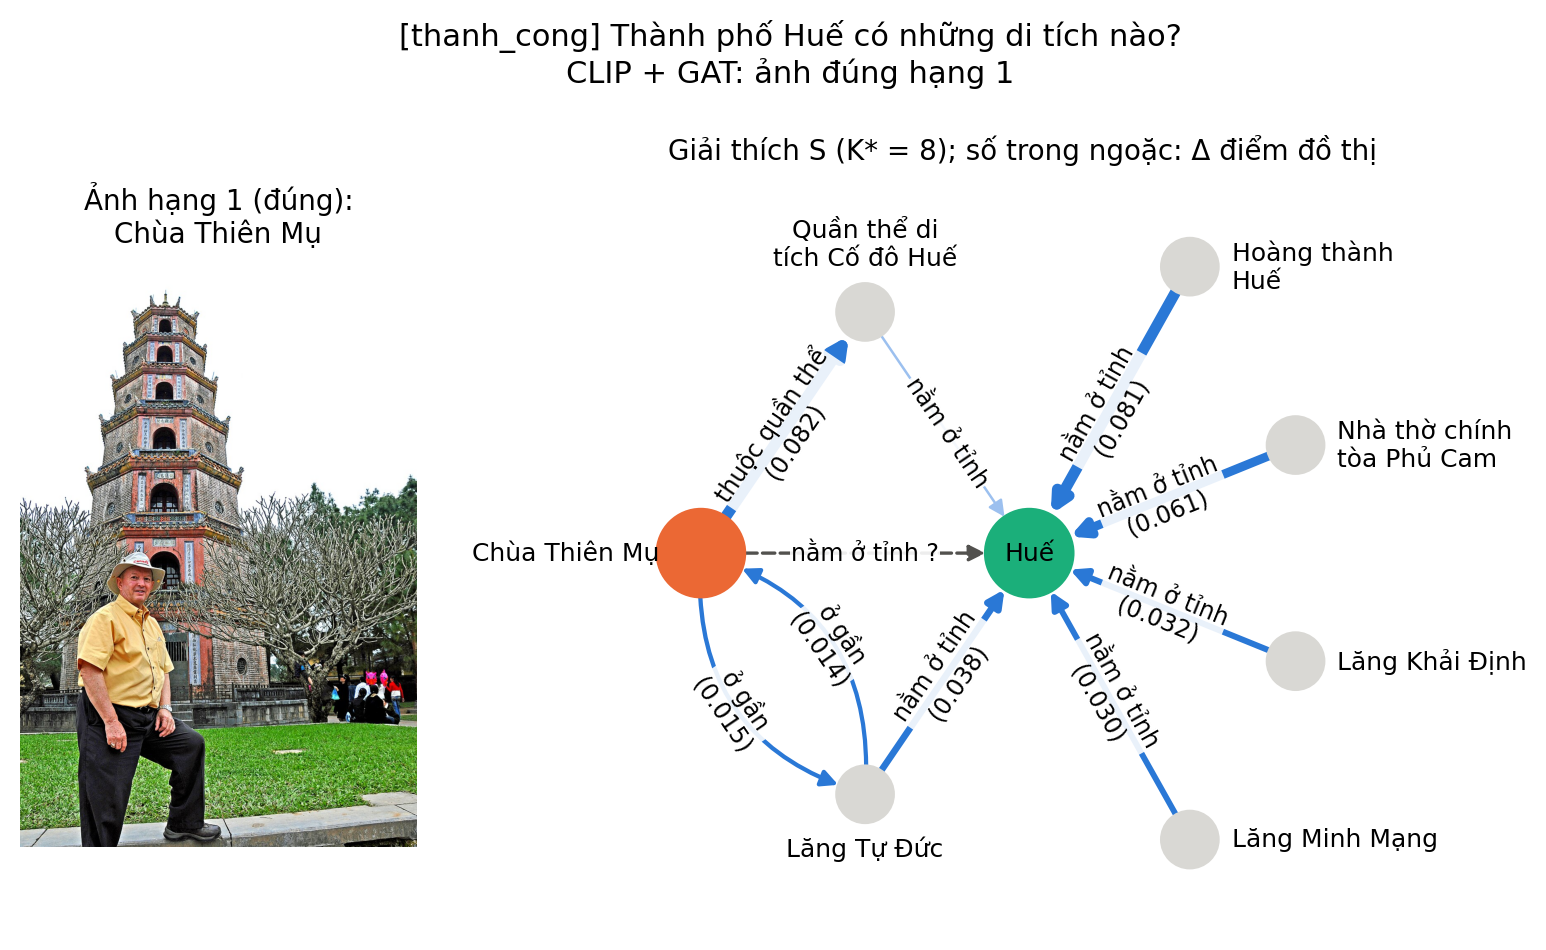
\includegraphics[width=0.8\textwidth]{figures/case_viheritage_gat_hue.png}
\caption{Ca thành công trên ViHeritage với GAT: truy vấn ``Thành phố Huế có những di tích nào?'' (thực thể neo Huế, nút xanh ngọc; ảnh trả về Chùa Thiên Mụ, nút cam; quan hệ \textit{nằm ở tỉnh} được hỏi, nét đứt). Nét đậm: 8 bộ ba giải thích, độ dày và số trong ngoặc là mức giảm điểm đồ thị khi che bộ ba đó; nét mảnh: bộ ba train nối bộ ba đứng đầu về Huế.}
\label{fig:case-viheritage}
\end{figure*}

Ca thành công điển hình ở Hình~\ref{fig:case-viheritage}: cả AdaMF và GAT đều trả về Chùa Thiên Mụ ở hạng 1 và cùng xếp bộ ba Chùa Thiên Mụ \textit{thuộc quần thể} Quần thể di tích Cố đô Huế lên đầu; bộ ba này nối với thực thể neo qua Quần thể di tích Cố đô Huế \textit{nằm ở tỉnh} Huế. Với AdaMF, đây là giải thích duy nhất ($K^\star = 1$, Fid+ 0.27 so với 0.06 ngẫu nhiên); với GAT, giải thích còn gồm các di tích khác \textit{nằm ở tỉnh} Huế (Fid+ 0.49 so với 0.01). Ca ``Đồng Nai có những địa danh nào đáng đến?'' với GAT trả về Vườn quốc gia Cát Tiên qua đường đi Cát Tiên \textit{nằm ở tỉnh} Lâm Đồng, Lâm Đồng \textit{giáp ranh} Đồng Nai. Năm ca thất bại của mỗi mô hình cho thấy bốn mẫu lỗi: (1) với truy vấn \textit{ở gần X}, mô hình trả về chính X (sáu trong mười ca thất bại), giống lỗi trả về thực thể neo trên DB15K; (2) bộ ba giải thích đúng nhưng không liên quan tới quan hệ được hỏi, ví dụ trả về Lăng Minh Mạng cho truy vấn tìm chùa vì bộ ba Lăng Minh Mạng \textit{nằm ở tỉnh} Huế; (3) lỗi dữ liệu Wikidata đi vào đường đi (Lăng Minh Mạng \textit{thuộc quần thể} Hoàng thành Huế); (4) hai danh hiệu di sản bị lẫn qua một thực thể mang cả hai nhãn (Cát Bà). Các ca thất bại cho thấy giải thích trung thành với mô hình nhưng không bảo đảm hợp lý theo kiến thức miền.

\section{Tổng hợp theo câu hỏi nghiên cứu}
\label{sec:cross-level-findings}

\begin{enumerate}
  \item \textbf{Cấp độ 1.} Trên Visual Genome, CLIP + GAT nâng MRR test từ 0.0611 lên 0.0718; khoảng 77\% mức tăng vẫn còn khi bỏ cạnh và 92\% khi xáo cạnh, nên phần lớn cải thiện đến từ phép biến đổi đặc trưng học được, cấu trúc cạnh đóng góp phần nhỏ. Giải thích bằng quan hệ trung thành với mô hình (Fid+ 0.118 so với 0.003 ngẫu nhiên) và xác nhận điều này: 75\% phần tử là cạnh \texttt{contains}, quan hệ giữa hai vật đóng góp ít hơn nhiều.
  \item \textbf{Cấp độ 2.} Đồ thị tri thức giúp rõ nhất ở truy vấn gián tiếp (DB15K gấp 6.6 lần, FB15K-237-IMG gấp 9.7 lần). Vai trò của cạnh thật được chứng minh trên DB15K nhưng không trên FB15K-237-IMG. GAT cấp 1 trên cùng pipeline ngang AdaMF.
  \item \textbf{Cấp độ 3.} Giải thích lấy từ can thiệp vào hàm xếp hạng có fidelity cao hơn ngẫu nhiên và heuristic ở mọi tập, và trên ViHeritage kết quả giữ khi kiểm chứng bằng huấn luyện lại; độ thưa 0.65 đến 0.80. Trên MMKG tiếng Việt tự xây, đồ thị vẫn giúp truy vấn gián tiếp và lợi ích phụ thuộc hoàn toàn vào cạnh thật.
\end{enumerate}

Báo cáo không so sánh MRR giữa các tập dữ liệu vì mỗi tập có không gian ứng viên, số truy vấn và mức độ phức tạp quan hệ khác nhau.

\chapter{Thảo luận}
\label{chap:discussion}

\section{Đồ thị giúp truy vấn ở đâu}
\label{sec:effectiveness-discussion}

Kết quả ở Chương~\ref{chap:results} cho thấy kết hợp CLIP với biểu diễn đồ thị cải thiện truy hồi trong các giao thức đã khảo sát. Tuy nhiên, mức tăng phản ánh đồng thời thông tin quan hệ, các thành phần học được và cách dung hợp điểm; cần phân tích riêng từng bộ dữ liệu thay vì xem mọi cải thiện là bằng chứng của suy luận qua cạnh.

Trên Visual Genome, MRR tăng từ 0.061149 lên $0.071817\pm0.000166$, tương ứng tăng tương đối khoảng 17.4\%. Kết quả phù hợp với giả thuyết scene graph bổ sung tín hiệu đối tượng và quan hệ cho biểu diễn ảnh toàn cục. Độ lệch chuẩn nhỏ cho thấy sự ổn định theo khởi tạo trong phạm vi giao thức, chưa chứng minh tổng quát hóa sang miền ảnh khác. GAT chỉ xếp hạng lại top 50 của CLIP, nên không đưa được ảnh đúng ngoài nhóm này vào top 50. Chất lượng truy hồi ban đầu vẫn giới hạn hiệu quả cuối cùng.

Trên DB15K, lợi ích tập trung vào truy vấn gián tiếp: MRR tăng từ 0.047527 lên 0.314268, khoảng 6.6 lần, trong khi truy vấn trực tiếp giữ thứ hạng CLIP theo thiết kế. Hai seed chọn $\alpha_{\mathrm{CLIP}}=0$ nhưng CLIP vẫn tạo top 1\,000 ảnh ứng viên; giá trị này không có nghĩa hệ thống hoạt động độc lập với CLIP. Trên FB15K-237-IMG, MRR gián tiếp tăng khoảng 9.7 lần và nhóm trực tiếp cũng cải thiện nhờ pipeline học mục tiêu truy hồi, lớp chiếu và biểu diễn dung hợp. Hai giao thức vì vậy không cho phép quy mức tăng trực tiếp cho cùng một cơ chế.

Trên ViHeritage, MRR gián tiếp của AdaMF và GAT đạt 0.219 và 0.258, so với 0.112 của CLIP; khoảng tin cậy chênh lệch của từng phương pháp với CLIP đều dương. Tuy nhiên, khoảng tin cậy GAT trừ AdaMF chứa 0 và $p=0.29$, nên chưa đủ bằng chứng kết luận GAT tốt hơn AdaMF trên test. Đồ thị giúp nhiều với quan hệ như \textit{thuộc quần thể}, \textit{danh hiệu di sản} và \textit{nằm ở tỉnh}, nhưng làm hại ở \textit{là một} và \textit{xây dựng vào thế kỷ}. Phân tích theo quan hệ cần thiết vì chỉ số gộp có thể che mất những nhóm truy vấn không được cải thiện.

\section{Mức tăng có thực sự đến từ cấu trúc quan hệ}
\label{sec:structural-contribution}

Hình~\ref{fig:ablation-all} cho thấy vai trò của cạnh khác nhau giữa các pipeline. Trên Visual Genome seed 2026, No-edge đạt MRR 0.069193, Random-edges đạt 0.070772 và Full Graph đạt 0.071655. Khoảng 77\% và 92\% mức tăng so với CLIP còn giữ lại khi bỏ hoặc xáo cạnh. Đây là tỷ lệ mô tả các lượt chạy, không phải phân rã nhân quả chính xác. No-edge giữ phép biến đổi học được và residual path, cho thấy biểu diễn có học đóng góp đáng kể ngay cả khi không truyền tin qua cạnh. Khoảng cách Full Graph--Random-edges chỉ 0.000883 MRR và mới quan sát ở một seed.

Trên DB15K seed 2027, đồ thị gốc cao hơn Shuffled Edges 0.098917 MRR tổng hợp và 0.169569 MRR gián tiếp. Kết quả hỗ trợ vai trò của quan hệ đúng ở cấp cấu hình. Tuy nhiên, Shuffled Edges vẫn có embedding học được và cơ chế dung hợp; việc nó vượt CLIP chưa cô lập tác dụng của phân phối bậc. No Edges bỏ huấn luyện và trả về CLIP, khác No-edge có học của Visual Genome. Random Graph cũng trả về CLIP vì validation chọn $\alpha_{\mathrm{CLIP}}=1$; đây là bằng chứng quy trình lựa chọn loại bỏ điểm đồ thị ngẫu nhiên, chưa đo tác hại khi buộc dùng điểm đó.

Trên FB15K-237-IMG, Random Graph và Shuffled Edges vẫn giữ khoảng 93.6\% MRR gián tiếp của đồ thị gốc. Các can thiệp thay neo train gián tiếp nhưng giữ giám sát trực tiếp và tham số dùng chung, nên phần lớn hiệu năng còn lại có thể liên quan đến biểu diễn và mục tiêu truy hồi. Trên ViHeritage, bỏ cạnh đưa MRR gián tiếp về gần CLIP, còn xáo cạnh làm kết quả thấp hơn CLIP. Các đối chứng này ủng hộ sự phụ thuộc vào liên kết đúng trong giao thức ViHeritage. Chưa nên quy khác biệt với FB15K cho riêng loss vì dữ liệu, chiều embedding và kiểu can thiệp cũng khác nhau.

\begin{figure}[!t]
\centering
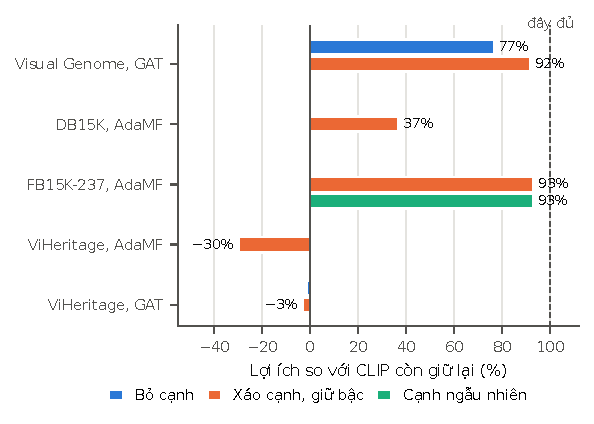
\includegraphics[width=\columnwidth]{figures/fig_ablation_gain_kept.pdf}
\caption{Phần lợi ích so với CLIP còn giữ lại khi bỏ, xáo hoặc thay ngẫu nhiên cạnh (mỗi biến thể một lần huấn luyện). Visual Genome dùng MRR toàn bộ test; các tập còn lại dùng MRR truy vấn gián tiếp. Cột không hiển thị là 0\%.}
\label{fig:ablation-all}
\end{figure}

\section{Độ tin cậy của giải thích}
\label{sec:xai-reliability}

\subsection{Bằng chứng can thiệp và giới hạn của phép xấp xỉ}

Bảng~\ref{tab:xai-all} cho thấy bỏ tập giải thích làm xác suất ảnh trả về giảm nhiều hơn bỏ cùng số phần tử ngẫu nhiên trên các bộ dữ liệu. Trên DB15K và FB15K, Fid+ trung bình đạt 0.511 và 0.335, so với 0.023 và 0.011 của đối chứng. Tuy nhiên, cần phân biệt che quan hệ trên GAT với học lại nhúng cục bộ của AdaMF. Phép thứ hai giữ các tham số khác cố định, đo chênh lệch giữa các bản học lại rồi chuyển chênh lệch sang điểm checkpoint; nó không tương đương huấn luyện lại toàn bộ mô hình sau khi xóa bộ ba.

Các artifact \code{D3_fidelity_mimic_summary.csv} ghi nhận Pearson giữa điểm học lại đủ bộ ba và điểm gốc khoảng 0.957 trên DB15K và 0.527 trên FB15K. Đây là kiểm tra đồng biến điểm qua truy vấn, chưa bảo đảm giữ nguyên thứ hạng hoặc phản ứng can thiệp. Kết quả ViHeritage mới bổ sung kiểm chứng mạnh hơn: huấn luyện lại AdaMF từ đầu sau khi bỏ bằng chứng cho Fid+ 0.327, cao hơn 0.180 khi bỏ ngẫu nhiên ($p=0.0002$). Dù hướng tác động được hỗ trợ, Spearman giữa Fid+ xấp xỉ và huấn luyện lại chỉ 0.32. Pearson điểm gốc--mimic trên DB15K/FB15K và Spearman tác động can thiệp trên ViHeritage đo hai khía cạnh khác nhau, không dùng thay thế nhau.

\subsection{Tính cần thiết, tính đủ và tính hợp lệ}

Fid+ đo tác động khi bỏ bằng chứng; Fid$-$ đo thay đổi khi chỉ giữ bằng chứng theo định nghĩa tại phần phương pháp. Fid$-$ âm cho biết xác suất tăng sau can thiệp, không phải tỷ lệ giải thích đúng. Với AdaMF ViHeritage, $K^\star=1$ cho Fid+ cao nhưng PS chỉ 0.144; một bộ ba nhạy với phép bỏ chưa đủ giữ dự đoán. Với $K=2$, PS tăng khoảng 0.68 nhưng giải thích bớt thưa. Vì vậy, chọn $K$ chỉ theo tính cần thiết có thể bỏ qua tính đủ.

Sparsity của DB15K và FB15K tại $K^\star$ khoảng 0.799 và 0.795, còn Visual Genome khoảng 0.647. Các tỷ lệ phải được đọc theo tập phần tử nền của từng bộ giải thích; với KG, mẫu số là tập bộ ba gắn với thực thể đang xét, không phải toàn KG. Bản tổng hợp dùng trung vị Fid$-$ và Fid làm nhiễu trong mỗi lượt chạy, trong khi artifact tổng hợp cũ có trung bình; khác biệt thống kê này cần được giữ rõ khi đối chiếu.

Validity cấu trúc đạt 100\% trong mẫu kiểm tra: bằng chứng thuộc đồ thị hợp lệ và không chồng lấn held-out ở các bộ KG. Điều này chưa bảo đảm đúng ngữ nghĩa. Đánh giá ViHeritage đã có 20 case, với bốn trên mười giải thích hợp lý ở mỗi mô hình, nhưng chỉ một lượt chấm có hỗ trợ AI và chưa có hệ số đồng thuận. Những bằng chứng này giúp nhận diện lỗi, chưa thay thế đánh giá độc lập nhiều người chấm.

\subsection{Ý nghĩa của các ca thành công và thất bại}

Ca Huế--Chùa Thiên Mụ ở Hình~\ref{fig:case-viheritage} minh họa đường đi có ý nghĩa qua Quần thể di tích Cố đô Huế. Ngược lại, các ca thất bại cho thấy mô hình có thể trả về chính thực thể neo, dựa vào bộ ba không liên quan đến quan hệ được hỏi hoặc tiếp nhận lỗi Wikidata. Trên FB15K, case quốc tịch liên quan Rick Rubin đưa ảnh đúng từ hạng CLIP 269 lên hạng 1, nhưng một phần bằng chứng chỉ thuộc lân cận United States of America và không nối về neo. Truy hồi đúng không đồng nghĩa mọi phần tử giải thích đều là một chuỗi suy luận trực tiếp.

Các giải thích vì vậy hữu ích để chẩn đoán mô hình và dữ liệu. Độ nhạy với can thiệp là bằng chứng về hành vi trong giao thức đã đo, chưa xác nhận tính đúng theo kiến thức miền hoặc quan hệ nhân quả ngoài mô hình. Kết quả XAI trên 500 truy vấn Visual Genome, 70 truy vấn mỗi bộ KG và 50/54 truy vấn ViHeritage cần được diễn giải theo phạm vi mẫu tương ứng.

\section{Chất lượng dữ liệu, chuyển giao và giới hạn}
\label{sec:limitations}

\subsection{Giá trị của xử lý dữ liệu}

Kiểm định DB15K phát hiện official validation có trùng lặp và chồng lấn lớn với train/test. Bản chia sạch ở Mục~\ref{sec:db15k-preprocessing} tạo validation từ official train và giữ nguyên official test, làm cơ sở chọn mô hình cho thí nghiệm mới. Kết quả này phải tách biệt với tái lập benchmark gốc. Trên FB15K, loại cụm ảnh trùng chéo thực thể và dùng mask cho 280 thực thể thiếu ảnh giảm nhập nhằng đầu vào; chúng chưa xác nhận mọi ánh xạ ảnh--thực thể đúng ngữ nghĩa. Bản chia không trùng ảnh cũng không đồng nghĩa tách biệt thực thể. Hạn chế về provenance và kiểm định ảnh được nêu tại Mục~\ref{sec:level2-data-contract}.

\subsection{Phạm vi chuyển giao sang ViHeritage}

ViHeritage đã có dữ liệu xử lý, kết quả truy hồi, ablation và kiểm chứng XAI; không còn ở giai đoạn thu thập sơ bộ. Phương pháp được cấu hình và huấn luyện trên bộ đích theo giao thức ở Mục~\ref{sec:level3-methodology}. Kết quả cho thấy khả năng áp dụng phương pháp sang miền di sản tiếng Việt, không chứng minh chuyển nguyên checkpoint DB15K/FB15K sang thực thể và quan hệ mới mà không thích nghi.

Đối chứng che hoàn toàn văn bản của AdaMF cho MRR gián tiếp 0.230, so với 0.219 của bản đầy đủ; khoảng tin cậy chênh lệch chứa 0. Kết quả cho thấy chưa quan sát thấy suy giảm khi bỏ văn bản trong giao thức này, hỗ trợ nhận định rằng lợi ích không chỉ phụ thuộc tên neo xuất hiện trong mô tả. Nó chưa xác định ảnh hưởng của mọi dạng chồng lấn ngữ nghĩa hoặc đủ để khẳng định văn bản hoàn toàn không đóng góp. Bộ dữ liệu chỉ có 318 bộ ba train và 54 truy vấn gián tiếp test, thiên về địa danh nổi tiếng và có khoảng 35\% bộ ba suy ra; các giới hạn này thu hẹp phạm vi tổng quát hóa.

\subsection{Giới hạn thiết kế thực nghiệm}

\begin{itemize}
  \item Ablation Visual Genome mới có seed 2026; các biến thể KG được chạy một lần. Độ lệch chuẩn của mô hình đầy đủ không thay thế được độ bất định của chênh lệch ablation. Các cấu hình chọn checkpoint và trọng số riêng nên chưa cô lập hoàn toàn một yếu tố.
  \item Shuffled Edges của DB15K và FB15K dùng validation/test để loại cạnh trùng. Quy trình ngăn chèn bộ ba giữ lại nhưng chưa hoàn toàn mù với test; đây là điều kiện của giao thức cần công bố.
  \item Các pipeline khác loss, chiều embedding, dữ liệu và ngân sách huấn luyện. Không so sánh trực tiếp MRR giữa các bộ để kết luận mô hình nào tốt hơn tổng quát.
  \item Trên Visual Genome, truy vấn mô tả vùng nhưng ứng viên là cả ảnh và chỉ có một ảnh đúng được gán nhãn; kết quả còn phụ thuộc mức đầy đủ của nhãn và giới hạn top 50.
  \item Câu hỏi ViHeritage và một số đánh giá ngữ nghĩa được xây dựng với hỗ trợ AI, chưa có đánh giá độc lập nhiều người chấm. Baseline FB15K giữa các lượt mô hình đầy đủ và ablation còn sai khác nhỏ, cần đối chiếu hạng truy vấn và cấu hình trước khi quy nguyên nhân.
\end{itemize}

\section{Hướng phát triển}
\label{sec:future-directions-discussion}

Ưu tiên tiếp theo là tăng độ chắc chắn của những kết luận đã có:
\begin{enumerate}
  \item Chạy thêm seed cho ablation, báo độ bất định của chênh lệch và bổ sung đối chứng giữ kiến trúc, ngân sách học và quy tắc dung hợp tương đương; thử sinh cạnh hoàn toàn không dùng test.
  \item Mở rộng kiểm chứng xấp xỉ XAI bằng huấn luyện lại hoặc can thiệp phù hợp mô hình gốc, đo cả điểm và thứ hạng; chọn $K^\star$ theo tính cần thiết, tính đủ và độ gọn.
  \item Bổ sung người chấm độc lập, phân biệt validity cấu trúc với ngữ nghĩa; kiểm tra các bộ ba và đường đi ở case thất bại để sửa dữ liệu hoặc cơ chế chấm điểm.
  \item Mở rộng ViHeritage và kiểm tra theo nhóm quan hệ; đánh giá quy tắc loại ảnh của thực thể neo khi truy vấn yêu cầu một thực thể khác, thay vì áp dụng loại neo cho mọi quan hệ. Đối chiếu sai khác baseline và giữ đầy đủ cấu hình, hạng truy vấn, checksum để tái lập.
\end{enumerate}


\chapter{Kết luận}
\label{chap:conclusion}

Đồ án đã hoàn thành ba cấp độ, từ truy hồi đa phương thức bằng CLIP, cải thiện xếp hạng bằng mô hình đồ thị đến đánh giá khả năng giải thích và áp dụng trên dữ liệu tự xây dựng. Kết quả cho thấy CLIP kết hợp GAT cải thiện MRR 17.4\% trên Visual Genome, trong khi Indirect MRR trên DB15K tăng khoảng 6.6 lần. Tuy nhiên, các thí nghiệm ablation cho thấy đóng góp của thông tin quan hệ khác nhau giữa các bộ dữ liệu. Các thí nghiệm can thiệp cũng xác nhận những quan hệ được chọn làm giải thích có ảnh hưởng đến kết quả truy hồi, dù không phải mọi giải thích đều hợp lý về mặt kiến thức.

Bên cạnh đó, nhóm đã xây dựng ViHeritage-MMKG và triển khai đầy đủ quy trình huấn luyện, truy hồi và giải thích trên dữ liệu di sản Việt Nam. Nhìn chung, đồ án cho thấy tiềm năng của việc kết hợp CLIP với mô hình đồ thị, đồng thời nhấn mạnh sự cần thiết của việc kiểm chứng cả hiệu quả truy hồi, đóng góp của thông tin quan hệ và độ tin cậy của giải thích.


% Hai bảng toàn khổ của phụ lục. Được \input trước tài liệu tham khảo (main.tex) để LaTeX đặt chúng ở đầu
% trang phụ lục; nếu khai báo trong phụ lục, bảng toàn khổ bị đẩy sang một trang riêng.
\begin{table*}[!t]
\centering
\normalsize
\renewcommand{\arraystretch}{0.95}
\caption{Siêu tham số huấn luyện}
\label{tab:hyperparameters}
\begin{tabularx}{\linewidth}{@{}L{3.4cm}YYYY@{}}
\toprule
Tham số & Visual Genome (GAT) & DB15K (AdaMF) & FB15K-237-IMG (AdaMF) & ViHeritage (AdaMF / GAT)\\
\midrule
Bộ mã hóa đóng băng & CLIP ViT-B/32 (OpenAI) & CLIP ViT-B/32 & CLIP ViT-B/32 & CLIP ViT-B/32; CLIP đa ngôn ngữ cho văn bản\\
Bộ mã hóa đồ thị & 2 tầng GAT có đặc trưng cạnh, 4 head $\times$ 32 chiều, dropout 0.2 & AdaMF (cấu trúc, ảnh, văn bản), MAT tắt & AdaMF, MAT tắt & AdaMF / GAT 2 tầng có đặc trưng cạnh\\
Bộ chấm điểm đồ thị & Cosine với nút ảnh & RotatE, \texttt{dim} 250, margin 12 & RotatE, \texttt{dim} 64 & RotatE, \texttt{dim} 50 / 100, margin 6\\
Hàm mất mát & Cross-entropy, 50 âm khó & Sigmoid tự đối kháng, 128 âm & Cross-entropy, 50 âm khó & Sigmoid tự đối kháng, 32 âm\\
Learning rate & $10^{-4}$ (AdamW, weight decay $10^{-4}$) & $10^{-4}$ & $10^{-4}$ & $5\times10^{-4}$ / $2\times10^{-3}$\\
Batch & 8 truy vấn & 256 bộ ba & 8 truy vấn & 64 bộ ba\\
Số epoch tối đa & 100 & 500 & 50 & 1\,500, patience 12\\
Tập ứng viên xếp hạng lại & Top-50 CLIP & Top-1\,000 CLIP & Top-1\,000 CLIP & Toàn bộ 88 ảnh test\\
$\alpha_{\mathrm{CLIP}}$ & 0.6 & 0.0 hoặc 0.1 & 0.1 & 0.0 / 0.0 hoặc 0.1\\
\bottomrule
\end{tabularx}
\end{table*}

\begin{table*}[!t]
\centering
\normalsize
\setlength{\tabcolsep}{4pt}
\caption{Phân công trách nhiệm của thành viên}
\label{tab:contributions}
\begin{tabularx}{\linewidth}{@{}lL{5.2cm}Y@{}}
\toprule
STT & Họ tên, MSSV & Nhiệm vụ chính\\
\midrule
1 & Chung Gia Khánh, 23120282 & Thiết kế kiến trúc tổng thể, audit kỹ thuật, kiểm thử triệt tiêu, biên tập báo cáo\\
2 & Lê Hoàng Mỹ Hạ, 23120038 & Tiền xử lý dữ liệu, kiểm soát rò rỉ, trích xuất đặc trưng CLIP\\
3 & Hàn Vũ Phương Uyên, 23120106 & Xây dựng scene graph, triển khai GAT, phân tích cấp độ 1\\
4 & Trần Gia Hiển, 23120123 & Triển khai AdaMF trên DB15K, FB15K-237-IMG và các đối chứng cấp độ 2\\
5 & Nguyễn An Nghiệp, 23127234 & Giải thích đồ thị, đánh giá XAI, dữ liệu MMKG tự xây\\
\bottomrule
\end{tabularx}
\end{table*}

\renderbibliography

\appendices
\chapter{Phụ lục bổ trợ}
\label{chap:appendices}

\section{Phụ lục A: Pipeline GAT trên Flickr30k Entities}
\label{app:flickr30k-pipeline}

\subsection{Xây dựng đồ thị}

Mỗi ảnh Flickr30k được biểu diễn bằng một đồ thị độc lập gồm một đỉnh ảnh và các đỉnh vùng được tạo từ bounding box của Flickr30k Entities. Đỉnh ảnh dùng embedding 512 chiều của toàn bộ ảnh; mỗi đỉnh vùng dùng embedding 512 chiều của phần ảnh được crop theo bounding box. Các đặc trưng được trích xuất bằng CLIP \texttt{ViT-B-32-quickgelu}, pretrained \texttt{openai}, và được giữ cố định.

Đồ thị sử dụng tám loại cạnh: \texttt{self}, \texttt{contains}, \texttt{in\_image}, \texttt{overlap}, \texttt{left\_of}, \texttt{right\_of}, \texttt{above} và \texttt{below}. Với mỗi vùng, pipeline tạo hai cạnh $v_{\mathrm{image}}\xrightarrow{\mathrm{contains}}v_{\mathrm{region}}$ và $v_{\mathrm{region}}\xrightarrow{\mathrm{in\_image}}v_{\mathrm{image}}$; đồng thời mỗi đỉnh được gán một self-loop.

Quan hệ giữa hai vùng được suy ra từ bounding box. Nếu diện tích giao của hai box lớn hơn 0, hai cạnh \texttt{overlap} ngược chiều được tạo. Nếu hai box không giao nhau và khoảng cách Euclidean giữa hai tâm nhỏ hơn 0.35 trong hệ tọa độ chuẩn hóa, trục có độ lệch lớn hơn quyết định cặp quan hệ \texttt{left\_of}/\texttt{right\_of} hoặc \texttt{above}/\texttt{below}. Không tạo cạnh không gian nếu khoảng cách lớn hơn hoặc bằng 0.35. Ngưỡng 0.35 là heuristic được hard-code trong pipeline, không phải siêu tham số được chọn trên validation. Loại cạnh được biểu diễn bằng vectơ one-hot 8 chiều.

Tập dữ liệu gồm 29\,783 đồ thị huấn luyện, 1\,000 đồ thị validation và 1\,000 đồ thị test. Số đỉnh trung bình tương ứng là 9.691, 9.595 và 9.339; khoảng min--max là $1$--$107$, $2$--$48$ và $1$--$44$. Số cạnh có hướng trung bình, đã bao gồm self-loop và các cạnh hai chiều, lần lượt là 90.543, 85.899 và 84.651; khoảng min--max là $1$--$6\,829$, $4$--$1\,504$ và $1$--$1\,129$.

Tần suất tám loại cạnh trên toàn bộ dữ liệu là: \texttt{overlap} (1\,258\,162), \texttt{self} (307\,558), \texttt{contains} (275\,775), \texttt{in\_image} (275\,775), \texttt{left\_of} (264\,124), \texttt{right\_of} (264\,124), \texttt{above} (110\,837) và \texttt{below} (110\,837).

Ví dụ, đồ thị của ảnh \texttt{1100214449} gồm một đỉnh ảnh và bốn đỉnh vùng tương ứng với \emph{boy}, \emph{fountain}, \emph{building} và \emph{striped shirt}. Đồ thị có 5 self-loop, 8 cạnh ảnh--vùng và 6 cạnh \texttt{overlap} có hướng. Ba cặp vùng giao nhau là \emph{boy--building}, \emph{boy--striped shirt} và \emph{building--striped shirt}, với một cạnh cho mỗi hướng.

\subsection{Kiến trúc GAT và image-root readout}

GAT gồm hai lớp. Lớp thứ nhất ánh xạ đặc trưng từ 512 xuống 256 chiều với hai attention head và \texttt{concat=False}; lớp thứ hai ánh xạ từ 256 về 512 chiều với một attention head. Mô hình không sử dụng dropout và không để GAT tự thêm self-loop vì self-loop đã được tạo trong dữ liệu. Trong một mini-batch, vị trí đỉnh ảnh của mỗi đồ thị được xác định bởi \texttt{batch.ptr[:-1]}. Embedding đỉnh ảnh sau GAT được cộng residual với CLIP image embedding ban đầu $x_i^{\text{image}}$, sau đó áp dụng LayerNorm và chuẩn hóa L2:
\begin{equation}
  h_{\text{graph}}^{\text{F30K}}(v_i)
  = \operatorname{L2Norm}\!\left(
      \operatorname{LayerNorm}\!\left(H_i^{(2)}[r_i] + x_i^{\text{image}}\right)
    \right).
  \label{eq:flickr-root-readout}
\end{equation}

Khác với Visual Genome, quan hệ trong đồ thị Flickr30k được suy ra từ hình học bounding box thay vì predicate ngữ nghĩa của scene graph. Vì vậy, Visual Genome biểu diễn trực tiếp các quan hệ như \emph{man--holding--microphone}, trong khi Flickr30k chủ yếu biểu diễn quan hệ không gian như \emph{overlap}, \emph{left of} và \emph{above}.


\subsection{Kết quả truy hồi}

Trên Flickr30k Entities, CLIP-only đạt R@1 0.6120, R@5 0.8240, R@10 0.8845 và MRR 0.7232. Kết quả CLIP + GAT qua ba seed được trình bày trong Bảng~\ref{tab:flickr30k-results}.

\begin{table*}[!t]
\centering
\small
\setlength{\tabcolsep}{4pt}
\caption{Hiệu năng truy vấn trên Flickr30k Entities}
\label{tab:flickr30k-results}
\begin{tabular}{lrrrr}
\toprule
Cấu hình & R@1 & R@5 & R@10 & MRR\\
\midrule
CLIP-only & 0.6120 & 0.8240 & 0.8845 & 0.7232\\
CLIP + GAT, seed 2026 & 0.7385 & 0.8920 & 0.9310 & 0.8251\\
CLIP + GAT, seed 2027 & 0.7410 & 0.8950 & 0.9340 & 0.8290\\
CLIP + GAT, seed 2028 & 0.7390 & 0.8940 & 0.9330 & 0.8278\\
\midrule
Trung bình & 0.7395 & 0.8937 & 0.9327 & 0.8273\\
Độ lệch chuẩn mẫu & 0.0013 & 0.0015 & 0.0015 & 0.0020\\
\bottomrule
\end{tabular}
\end{table*}

\subsection{Ablation}

Hai đối chứng No-edges và Random-edges được đánh giá trên seed \texttt{2026}. No-edges chỉ giữ self-loop, trong khi Random-edges thay thế liên kết đúng bằng liên kết ngẫu nhiên.

\begin{table*}[!t]
\centering
\small
\setlength{\tabcolsep}{4pt}
\caption{Ablation trên Flickr30k Entities, seed 2026}
\label{tab:flickr30k-ablation}
\begin{tabular}{lrrrr}
\toprule
Cấu hình & R@1 & R@5 & R@10 & MRR\\
\midrule
CLIP-only & 0.6120 & 0.8240 & 0.8845 & 0.7232\\
No-edges / Adapter & 0.6840 & 0.8520 & 0.9010 & 0.7810\\
Random-edges & 0.6380 & 0.8310 & 0.8890 & 0.7450\\
Full Graph & 0.7385 & 0.8920 & 0.9310 & 0.8251\\
\bottomrule
\end{tabular}
\end{table*}

Kết quả này cho thấy không thể đồng nhất No-edges với CLIP-only hoặc quy toàn bộ mức tăng cho cấu trúc cạnh.

\section{Phụ lục B: Cấu hình siêu tham số và tài nguyên tính toán}
\label{app:hyperparameters}

Bảng~\ref{tab:hyperparameters} liệt kê chi tiết các siêu tham số được sử dụng để huấn luyện mô hình ở từng cấp độ thực nghiệm:

\begin{table*}[!t]
\centering
\small
\renewcommand{\arraystretch}{0.95}
\caption{Bảng tổng hợp siêu tham số huấn luyện của các mô hình}
\label{tab:hyperparameters}
\begin{tabularx}{\textwidth}{L{4.0cm}L{3.5cm}L{3.5cm}Y}
\toprule
\textbf{Tham số / Cấu hình} & \textbf{Level 1 (GAT)} & \textbf{Level 2 (AdaMF)} & \textbf{Ghi chú}\\
\midrule
Backbone thị giác & ViT-B/32 (OpenCLIP) & ViT-B/32 (OpenCLIP) & Đóng băng toàn bộ trọng số\\
Kích thước nhúng ($d$) & 512 & 512 & Đồng nhất không gian CLIP\\
Số lớp GNN & 2 lớp GAT & 2 tầng Transformer & Truyền thông điệp cục bộ\\
Hidden dimension & 128 & 256 & Chiếu không gian trung gian\\
Số attention heads & 4 heads & 4 heads & Đa cơ chế chú ý\\
Tỷ lệ Dropout & 0.2 & 0.1 & Phòng chống quá khớp\\
Hàm tối ưu & AdamW & AdamW & Weight decay = $1\text{e-}4$\\
Learning rate & $1\text{e-}3$ & $5\text{e-}4$ & Giảm theo Cosine Annealing\\
Số Epoch tối đa & 50 & 500 (Early stop = 8) & Dừng sớm theo Validation\\
Trọng số kết hợp $\alpha_{\text{CLIP}}$ & 0.6 (trên VG) & 0.2 (trên DB15K) & Khóa trên Validation\\
\bottomrule
\end{tabularx}
\end{table*}

\section{Phụ lục C: Hướng dẫn tái lập thực nghiệm}
\label{app:reproduction}

Quy trình tái lập các kết quả thực nghiệm từ mã nguồn và dữ liệu đã chuẩn hóa được tóm tắt qua các bước chuẩn:

\begin{lstlisting}[language=bash,caption={Các bước tái lập thực nghiệm trên môi trường GPU}]
# 1. Khoi tao moi truong ao va cai dat thu vien
python3 -m venv venv && source venv/bin/activate
pip install torch torchvision --index-url https://download.pytorch.org/whl/cu121
pip install torch_geometric pyarrow duckdb pandas scikit-learn transformers

# 2. Xac thuc ma bam du lieu va checkpoint
sha256sum -c reference/model_handoff_manifest.json

# 3. Tai lap ket qua suy luan Level 1 (Flickr30k)
python src/gml_v1/evaluate_gat.py --seed 2026 --checkpoint model/gat_v1/seed_2026/best.pt

# 4. Tai lap ket qua suy luan Level 2 (DB15K AdaMF seed 2027)
python src/gml_v2/evaluate_adamf.py --dataset DB15K --seed 2027 --alpha 0.2
\end{lstlisting}

\section{Phụ lục D: Phân công trách nhiệm của thành viên}
\label{app:contributions}

Bảng~\ref{tab:contributions} ghi nhận vai trò chính của từng thành viên trong nhóm đồ án:

\begin{table*}[!t]
\centering
\small
\renewcommand{\arraystretch}{0.95}
\caption{Phân công trách nhiệm của thành viên}
\label{tab:contributions}
\begin{tabularx}{\textwidth}{C{1.0cm}L{3.4cm}L{2.5cm}Y}
\toprule
\textbf{STT} & \textbf{Họ và tên} & \textbf{MSSV} & \textbf{Nhiệm vụ chính phụ trách}\\
\midrule
1 & Chung Gia Khánh & 23120282 & Thiết kế kiến trúc tổng thể, audit kỹ thuật, kiểm thử triệt tiêu và biên tập báo cáo\\
2 & Lê Hoàng Mỹ Hạ & 23120038 & Tiền xử lý dữ liệu, kiểm soát rò rỉ và trích xuất đặc trưng CLIP\\
3 & Hàn Vũ Phương Uyên & 23120106 & Xây dựng scene graph, triển khai GAT và phân tích Level 1\\
4 & Trần Gia Hiển & 23120123 & Triển khai AdaMF, DB15K, FB15K-237-IMG và các đối chứng Level 2\\
5 & Nguyễn An Nghiệp & 23127234 & Triển khai giải thích đồ thị, đánh giá XAI và dữ liệu MMKG tự xây\\
\bottomrule
\end{tabularx}
\end{table*}


\end{document}
